% Template for the Journal of Computational Science and Applications (JCSA)
% Published by the University of Lahore -- ISSN 2710-3102
% Official author guidelines: https://journals.uol.edu.pk/JCSA/Author-Guideline
\documentclass[twoside,twocolumn,10pt]{article}
\usepackage{fancyhdr}
\usepackage{geometry}
\usepackage{multicol}
\usepackage{abstract}
\usepackage{graphicx}
\graphicspath{{imagenes/}}
\usepackage{caption}
\usepackage{threeparttable}
\usepackage{titlesec}
\usepackage{ragged2e}  % Provides the justifying command
\usepackage{amssymb}  % For additional symbols
\usepackage{parskip}  % Automatically handles paragraph spacing
\usepackage{amsmath}  % For advanced math environments
\usepackage{newtxtext}  % Times New Roman font
\usepackage{booktabs}  % For improved table appearance
\usepackage{array}     % For customizing table columns
\usepackage[spanish]{babel}
\usepackage[
	backend=biber,
	style=chem-acs, 	% Aplica el estilo compacto de revistas científicas
	articletitle=false,
	maxnames=4,        % Si hay más de 4 autores, usa el primero seguido de "et al."
	minnames=1
]{biblatex}
\usepackage[version=4]{mhchem} %Use Chemical Notation
\usepackage{url}
\addbibresource{references.bib}
% The starting page number is normally assigned by the editorial office
% once the article is scheduled into a specific issue. Authors can leave
% this at 1; production will update it if required.
\setcounter{page}{1}

% Define custom column types for better alignment and spacing
\newcolumntype{L}[1]{>{\raggedright\arraybackslash}p{#1}} % Left aligned column
\newcolumntype{C}[1]{>{\centering\arraybackslash}p{#1}}   % Center aligned column
\newcolumntype{R}[1]{>{\raggedleft\arraybackslash}p{#1}}  % Right aligned column

\usepackage[font=footnotesize, labelfont=bf, justification=raggedright, format=plain]{caption}

\captionsetup[table]{
    labelsep=period,               % Period after label for tables
    justification=raggedright      % Ensure left alignment of captions
}

\captionsetup[figure]{
    labelsep=period,               % Period after label for figures
    justification=raggedright      % Ensure left alignment of captions
}

% Set page margins
\geometry{
    letterpaper,
    left=0.8in,
    right=0.8in,
    top=1in,
    bottom=1in
}

% Increase space between columns
\setlength{\columnsep}{20pt}

% Define the centred abstract heading
\renewcommand{\abstractname}{\hspace{1.3em}\textbf{Resumen}}

\titleformat{\section}{\large\bfseries\uppercase}{\thesection.}{1em}{}

\titleformat{\subsection}{\normalfont\bfseries\flushleft}{\thesubsection.}{1em}{}

\titleformat{\subsubsection}{\normalfont\bfseries\itshape\flushleft}{\thesubsubsection}{1em}{}

% Set font sizes for abstract
\renewcommand{\abstractnamefont}{\normalfont\fontsize{14}{20}\bfseries}
\renewcommand{\absnamepos}{flushleft}
\renewcommand{\abstracttextfont}{\normalfont\fontsize{11}{13}\selectfont}

% Keywords environment
\newcommand{\keywordsname}{Palabras clave}
\newenvironment{keywords}
  {\par\noindent\hspace{2em}\textbf{\keywordsname:}}
  {\par}

\hyphenpenalty=10000
\exhyphenpenalty=10000
\sloppy

% Set up header and footer styles
\pagestyle{fancy}
\fancyhf{}  % Clear default header and footer

% Odd page headers -- running form of the title
\fancyhead[C]{\small Reacciones de alcanos, alquenos y cicloalquenos}

% Even page headers -- first author's surname and year
\fancyhead[CE]{\small M\'endez Castellanos et al. (2026)}

% Footer: Page numbers only (on all pages except the first one)
\fancyfoot[C]{\thepage}

% First page custom header/footer
\fancypagestyle{firstpage}{
  \fancyhf{}  % Clear header and footer
  \fancyhead[LO]{\small Ingeniería Ambiental, FAMARENA-UD}  % Left header for first page
  \fancyhead[RO]{\small QUIMORG 2026-III}  % Right header for first page
  \fancyfoot[L]{\footnotesize Impreso: \today \\\textsuperscript{*}Corresponding Author: Jorge Nicol\'as M\'endez Castellanos \textless correo institucional\textgreater}
   \fancyfoot[R]{\footnotesize \copyright\ 2026 por los Autores. Publicado para proyecto final,\\\textsuperscript{*} bajo protección de difusión }
  \renewcommand{\headrulewidth}{0.4pt}  % Add header line
  \renewcommand{\footrulewidth}{0.4pt}  % Add footer line
}

\title{\fontsize{16}{20}\selectfont\textbf{An\'alisis gr\'afico y estad\'istico de reacciones y obtenciones de alcanos, alquenos y cicloalquenos}}
\author{
    \fontsize{12}{14}\selectfont
    Jorge Nicol\'as M\'endez Castellanos\textsuperscript{1*}, Laura Alejandra Parra\textsuperscript{1}, Gabriela Santamar\'ia\textsuperscript{1}\\[1ex]
    \fontsize{12}{14}\selectfont
    \textsuperscript{1}Ingenier\'ia Ambiental, Facultad de Medio Ambiente y Recursos Naturales,\\ Universidad Distrital Francisco Jos\'e de Caldas, Bogot\'a, Colombia \\
    C\'odigos estudiantiles: 20241180048, 20252180055, 20252180048
}
\date{}

\begin{document}

\twocolumn[
\begin{@twocolumnfalse}
\vspace{-0.5cm}  % Adjust spacing as needed between header and "Research Article"
\raggedright

{\fontsize{11}{13}\selectfont{Art\'iculo de investigaci\'on}}
\vspace{-0.8cm}  % Adjust spacing between "Research Article" and title

% Now, insert the title and the author information
\maketitle

\thispagestyle{firstpage} % Apply custom header/footer for first page
\begin{abstract}
\fontsize{11}{13}\selectfont
\vspace{1em}
\justifying
Se analizaron gr\'afica y estad\'isticamente 200 registros de reacciones y obtenciones de diez hidrocarburos (cinco alcanos, tres alquenos y dos cicloalquenos), con diez reacciones y diez obtenciones por sustancia, junto con ocho propiedades fisicoqu\'imicas de la sustancia asociada. Los datos se limpiaron, clasificaron y codificaron en Python (Google Colab) y se exploraron con mapas de calor de la correlaci\'on de Spearman, la $V$ de Cram\'er y la raz\'on de correlaci\'on $\eta$; despu\'es se evidenciaron con gr\'aficas de tendencia y de probabilidad condicional. El punto de ebullici\'on aument\'o con el peso molecular ($\rho=0{,}82$) y se relacion\'o casi linealmente con el logaritmo de la presi\'on de vapor ($\rho=-0{,}99$). La familia de reacci\'on se asoci\'o con el medio ($V=0{,}53$), el catalizador ($V=0{,}47$) y el solvente ($V=0{,}45$), con patrones coherentes con los mecanismos conocidos: eliminaci\'on en medio b\'asico (59\,\%) y sustituci\'on radicalaria en medio apolar (79\,\%). La temperatura de reacci\'on mostr\'o dos reg\'imenes: 51,5\,\% de los registros a 40\,\textdegree C o menos y un grupo t\'ermico entre 400 y 800\,\textdegree C. Las reacciones y las obtenciones no difirieron en la temperatura mediana ($p=0{,}88$), pero s\'i en el tipo de transformaci\'on ($V=0{,}76$) y en la dispersi\'on de la temperatura ($p=2{,}5\times10^{-5}$). Se concluye que el mecanismo y el grupo funcional, y no la sustancia de partida, determinan las condiciones de reacci\'on.

\vspace{-0.1cm}
\noindent\textbf{Palabras clave:}
 alcanos, alquenos, cicloalquenos, correlaci\'on de Spearman, $V$ de Cram\'er, probabilidad condicional.

\end{abstract}

\vspace{1cm}
\end{@twocolumnfalse}
]
\section{Introducción}
\fontsize{12}{14}\selectfont
Los alcanos, los alquenos y los cicloalquenos son las familias de hidrocarburos m\'as simples de la qu\'imica org\'anica y, a la vez, la materia prima de combustibles, solventes y de buena parte de la industria qu\'imica. Para la ingenier\'ia ambiental su estudio es relevante porque la volatilidad, la solubilidad en agua y la reactividad de estas sustancias determinan c\'omo se distribuyen y se transforman cuando llegan al aire, al agua o al suelo \cite{Clayden2012,McMurry2016}.

Las propiedades f\'isicas de un hidrocarburo dependen de su tama\~no y de su forma, mientras que las condiciones con que se transforma (catalizador, solvente, medio y temperatura) dependen del mecanismo de la reacci\'on. Ambas ideas se ense\~nan por separado en el curso, pero rara vez se contrastan con un conjunto grande de datos. Este trabajo las pone a prueba con una base de 200 registros: diez sustancias consultadas, cada una con diez reacciones (la sustancia como reactante) y diez obtenciones (la sustancia como producto), m\'as las propiedades de la sustancia asociada a cada registro.

El objetivo es identificar, mediante un an\'alisis gr\'afico y estad\'istico, qu\'e variables se relacionan entre s\'i y explicar esas relaciones con la qu\'imica de los compuestos. Se plantearon cuatro hip\'otesis antes de analizar: (H1) el peso molecular controla el punto de ebullici\'on y la presi\'on de vapor; (H2) el tipo de reacci\'on se asocia con el medio, el catalizador y el solvente; (H3) la temperatura de reacci\'on depende de la familia de reacci\'on y del catalizador; y (H4) las reacciones y las obtenciones no se hacen en las mismas condiciones.

El documento se organiza as\'i: la secci\'on 2 resume el marco te\'orico, la secci\'on 3 describe los datos y los m\'etodos, la secci\'on 4 presenta y discute los resultados y la secci\'on 5 expone las conclusiones.

\section{Revisión Literatura}
\subsection{Propiedades f\'isicas de los hidrocarburos}
Los alcanos y alquenos son moléculas apolares o muy poco polares, por lo que las fuerzas que las mantienen unidas en fase l\'iquida son las de dispersi\'on de London, que crecen con el n\'umero de electrones y con el \'area de contacto entre moléculas \cite{Clayden2012}. De ah\'i se derivan dos regularidades cl\'asicas: en una serie hom\'ologa el punto de ebullici\'on aumenta de forma regular con cada grupo $-\mathrm{CH_2}-$, y la ramificaci\'on lo reduce porque disminuye la superficie de contacto \cite{McMurry2016}. La presi\'on de vapor y el punto de ebullici\'on est\'an ligados por la ecuaci\'on de Clausius-Clapeyron, $\ln P=-\Delta H_{vap}/(RT)+C$: a mayor temperatura de ebullici\'on, menor presi\'on de vapor a temperatura ambiente \cite{Atkins2014}.

\subsection{Reactividad de alcanos y alquenos}
Los alcanos, sin grupos funcionales, reaccionan sobre todo por mecanismos radicalarios (halogenaci\'on con luz ultravioleta), por combusti\'on y por craqueo o isomerizaci\'on a alta temperatura con catalizadores \'acidos o met\'alicos. Los alquenos, en cambio, reaccionan en el doble enlace mediante adici\'on electrof\'ilica, hidrogenaci\'on cat\'alitica, oxidaci\'on y metátesis, y se obtienen por reacciones de eliminaci\'on (E1 o E2) y por hidrogenaci\'on parcial de alquinos \cite{Clayden2012,McMurry2016}. Estas rutas explican por qu\'e cada familia de reacci\'on se asocia a un tipo de medio, de catalizador y de temperatura, que es la idea que se verifica en este trabajo.

\subsection{Medidas de asociaci\'on y visualizaci\'on}
Para variables num\'ericas con distribuci\'on asim\'etrica o valores at\'ipicos se prefiere la correlaci\'on de rangos de Spearman \cite{Spearman1904}. Entre variables categ\'oricas se usa la $V$ de Cram\'er \cite{Cramer1946}, en su versi\'on corregida por sesgo \cite{Bergsma2013}, y para comparar una variable num\'erica entre grupos las pruebas no param\'etricas de Kruskal-Wallis \cite{Kruskal1952} y Mann-Whitney \cite{Mann1947}. La elecci\'on del tipo de gr\'afico sigue el criterio de la gu\'ia de Yi \cite{Yi2019}: se escoge seg\'un el rol del gr\'afico y el tipo de datos.

\section{Metodología}
\subsection{Descripci\'on de los datos}
Se consultaron en CAS SciFinder \cite{SciFinder} diez sustancias: pentano, isopentano, hexano, heptano, octano, pent-2-eno, 2-metilpent-2-eno, hex-1-eno, ciclopropeno y ciclobuteno. Para cada una se registraron diez reacciones y diez obtenciones (200 filas) con catalizador, reactivos, solvente, temperatura, medio (\'acido, b\'asico, neutro o apolar), productos, nombre y tipo de reacci\'on. A la sustancia asociada de cada fila (el producto principal en una reacci\'on y el reactante principal en una obtenci\'on) se le consultaron el peso molecular (PM), los puntos de fusi\'on ($T_f$) y de ebullici\'on ($T_{eb}$), la densidad, el pKa, el momento dipolar ($\mu$), la solubilidad en agua y la presi\'on de vapor ($P_{vap}$).

\subsection{Limpieza, clasificaci\'on y codificaci\'on}
El an\'alisis se hizo en Python \cite{Harris2020,McKinney2010,Virtanen2020} con las gr\'aficas de Matplotlib y Seaborn \cite{Hunter2007,Waskom2021} en un cuaderno de Google Colab. Primero se reemplaz\'o el gui\'on que marcaba datos no disponibles por valores vac\'ios y se convirtieron a n\'umero las columnas que hab\'ian quedado como texto; la solubilidad se separ\'o en el valor num\'erico y la categor\'ia cualitativa (\textit{miscible} o \textit{soluble}). El pKa tiene 71,5\,\% de datos vac\'ios (57 de 200) y se excluy\'o de las correlaciones. Los dem\'as vac\'ios (8\,\% en $T_{eb}$, 11\,\% en solubilidad y 5,5\,\% en $P_{vap}$) corresponden a propiedades que no existen, por ejemplo el punto de ebullici\'on de una sal que se descompone, y no se rellenaron.

Las variables se clasificaron seg\'un la tabla~\ref{tab:variables}. Como la tabla original tiene demasiadas categor\'ias para 200 filas, el tipo de reacci\'on se agrup\'o en nueve familias (adici\'on, oxidaci\'on, reducci\'on e hidrogenaci\'on, eliminaci\'on, sustituci\'on, isomerizaci\'on, ciclaci\'on, hidrogen\'olisis y craqueo, y acoplamiento o met\'atesis), el catalizador en siete categor\'ias seg\'un su naturaleza qu\'imica y el solvente en cuatro seg\'un su polaridad. La temperatura se dividi\'o en cinco rangos y la solubilidad en una escala ordinal de cinco clases. Despu\'es las categor\'ias se codificaron con enteros y se guard\'o una leyenda de c\'odigos.

\begin{table}[htpb]
	\centering
	\footnotesize
	\begin{tabular}{|L{0.17\columnwidth}|L{0.40\columnwidth}|L{0.26\columnwidth}|}
		\hline
		\textbf{Tipo} & \textbf{Variables} & \textbf{An\'alisis} \\
		\hline
		Nominal & sustancia, clase, consulta, medio, familia, catalizador, solvente & Frecuencias, $V$ de Cram\'er, $\chi^2$ \\
		\hline
		Ordinal & rango de temperatura, clase de solubilidad & Frecuencias \\
		\hline
		Num\'erica & $T_{rxn}$, PM, $T_f$, $T_{eb}$, densidad, $\mu$, solubilidad, $P_{vap}$ & Spearman, Kruskal-Wallis, Mann-Whitney \\
		\hline
	\end{tabular}
	\captionsetup{width=\columnwidth, justification=justified}
	\caption{Clasificaci\'on de las variables y medida usada con cada tipo.}
	\label{tab:variables}
\end{table}

\subsection{Medidas de asociaci\'on}
Entre variables num\'ericas se calcul\'o el coeficiente $\rho$ de Spearman, que mide si la relaci\'on es mon\'otona (var\'ia entre $-1$ y $+1$). Entre variables categ\'oricas se calcul\'o la $V$ de Cram\'er con la correcci\'on de sesgo de Bergsma \cite{Bergsma2013}:
\begin{equation}
\begin{split}
V&=\sqrt{\dfrac{\tilde{\varphi}^2}{\min(\tilde{k}-1,\,\tilde{r}-1)}},\\
\tilde{\varphi}^2&=\max\!\left(0,\dfrac{\chi^2}{n}-\dfrac{(k-1)(r-1)}{n-1}\right)
\end{split}
\end{equation}
donde $n$ es el n\'umero de datos, $r$ y $k$ son las categor\'ias de cada variable, y $\tilde{r}$ y $\tilde{k}$ sus versiones corregidas. $V$ toma valores entre 0 y 1; se interpret\'o con los umbrales de Cohen \cite{Cohen1988} (menor que 0,1 despreciable, 0,1--0,3 d\'ebil, 0,3--0,5 moderada y mayor que 0,5 fuerte). Para una variable categ\'orica contra una num\'erica se us\'o la raz\'on de correlaci\'on
\begin{equation}
\eta=\sqrt{\dfrac{\sum_g n_g(\bar{x}_g-\bar{x})^2}{\sum_i (x_i-\bar{x})^2}}
\end{equation}
cuyo cuadrado es la fracci\'on de la varianza explicada por el grupo. Los tres resultados se muestran primero como mapas de calor, que sirven para detectar qu\'e relaciones merecen una gr\'afica propia.

\subsection{Contraste de hip\'otesis y reproducibilidad}
Cada hip\'otesis se contrast\'o con una prueba no param\'etrica porque las variables son asim\'etricas y los grupos peque\~nos: Spearman (H1), chi-cuadrado con $V$ de Cram\'er (H2), Kruskal-Wallis con el tama\~no de efecto $\varepsilon^2=(H-k+1)/(n-k)$ \cite{Tomczak2014} (H3), y Mann-Whitney, Levene con centro en la mediana \cite{Brown1974} y chi-cuadrado (H4). Se rechaz\'o la hip\'otesis nula cuando $p<0{,}05$. Los valores at\'ipicos se identificaron con la regla del rango intercuart\'ilico, es decir, valores menores que $Q_1-1{,}5\,\mathrm{IQR}$ o mayores que $Q_3+1{,}5\,\mathrm{IQR}$. El cuaderno, la base y las figuras est\'an en el repositorio del proyecto en GitHub [completar enlace].

\section{Resultados y Discusión}
\subsection{Descripci\'on general}
El medio m\'as frecuente es el neutro (33,5\,\%), seguido del apolar (23\,\%), el b\'asico (22\,\%) y el \'acido (21,5\,\%). La familia m\'as com\'un es la eliminaci\'on (46 de 200 registros), seguida de la reducci\'on e hidrogenaci\'on (39) y la oxidaci\'on (30). La mitad de los registros (101) no usa catalizador y, entre los catalizados, predomina el metal soportado (46). Adem\'as, 51,5\,\% de los registros ocurre a 40\,\textdegree C o menos, de modo que la distribuci\'on de la temperatura est\'a muy concentrada cerca de la temperatura ambiente.

\subsection{Mapas de calor}
En la figura~\ref{fig:spearman} se ven dos bloques. Las propiedades f\'isicas est\'an muy correlacionadas entre s\'i, con la pareja m\'as fuerte entre presi\'on de vapor y punto de ebullici\'on ($\rho=-0{,}99$), seguida de PM y punto de ebullici\'on ($\rho=0{,}82$) y de PM y presi\'on de vapor ($\rho=-0{,}80$). En cambio, la temperatura de reacci\'on casi no se correlaciona con las propiedades f\'isicas ($|\rho|<0{,}2$, salvo $\rho=-0{,}32$ con el momento dipolar), lo cual es coherente con que dependa del mecanismo y no del tama\~no de la mol\'ecula asociada.

\begin{figure}[!htbp]
\centering
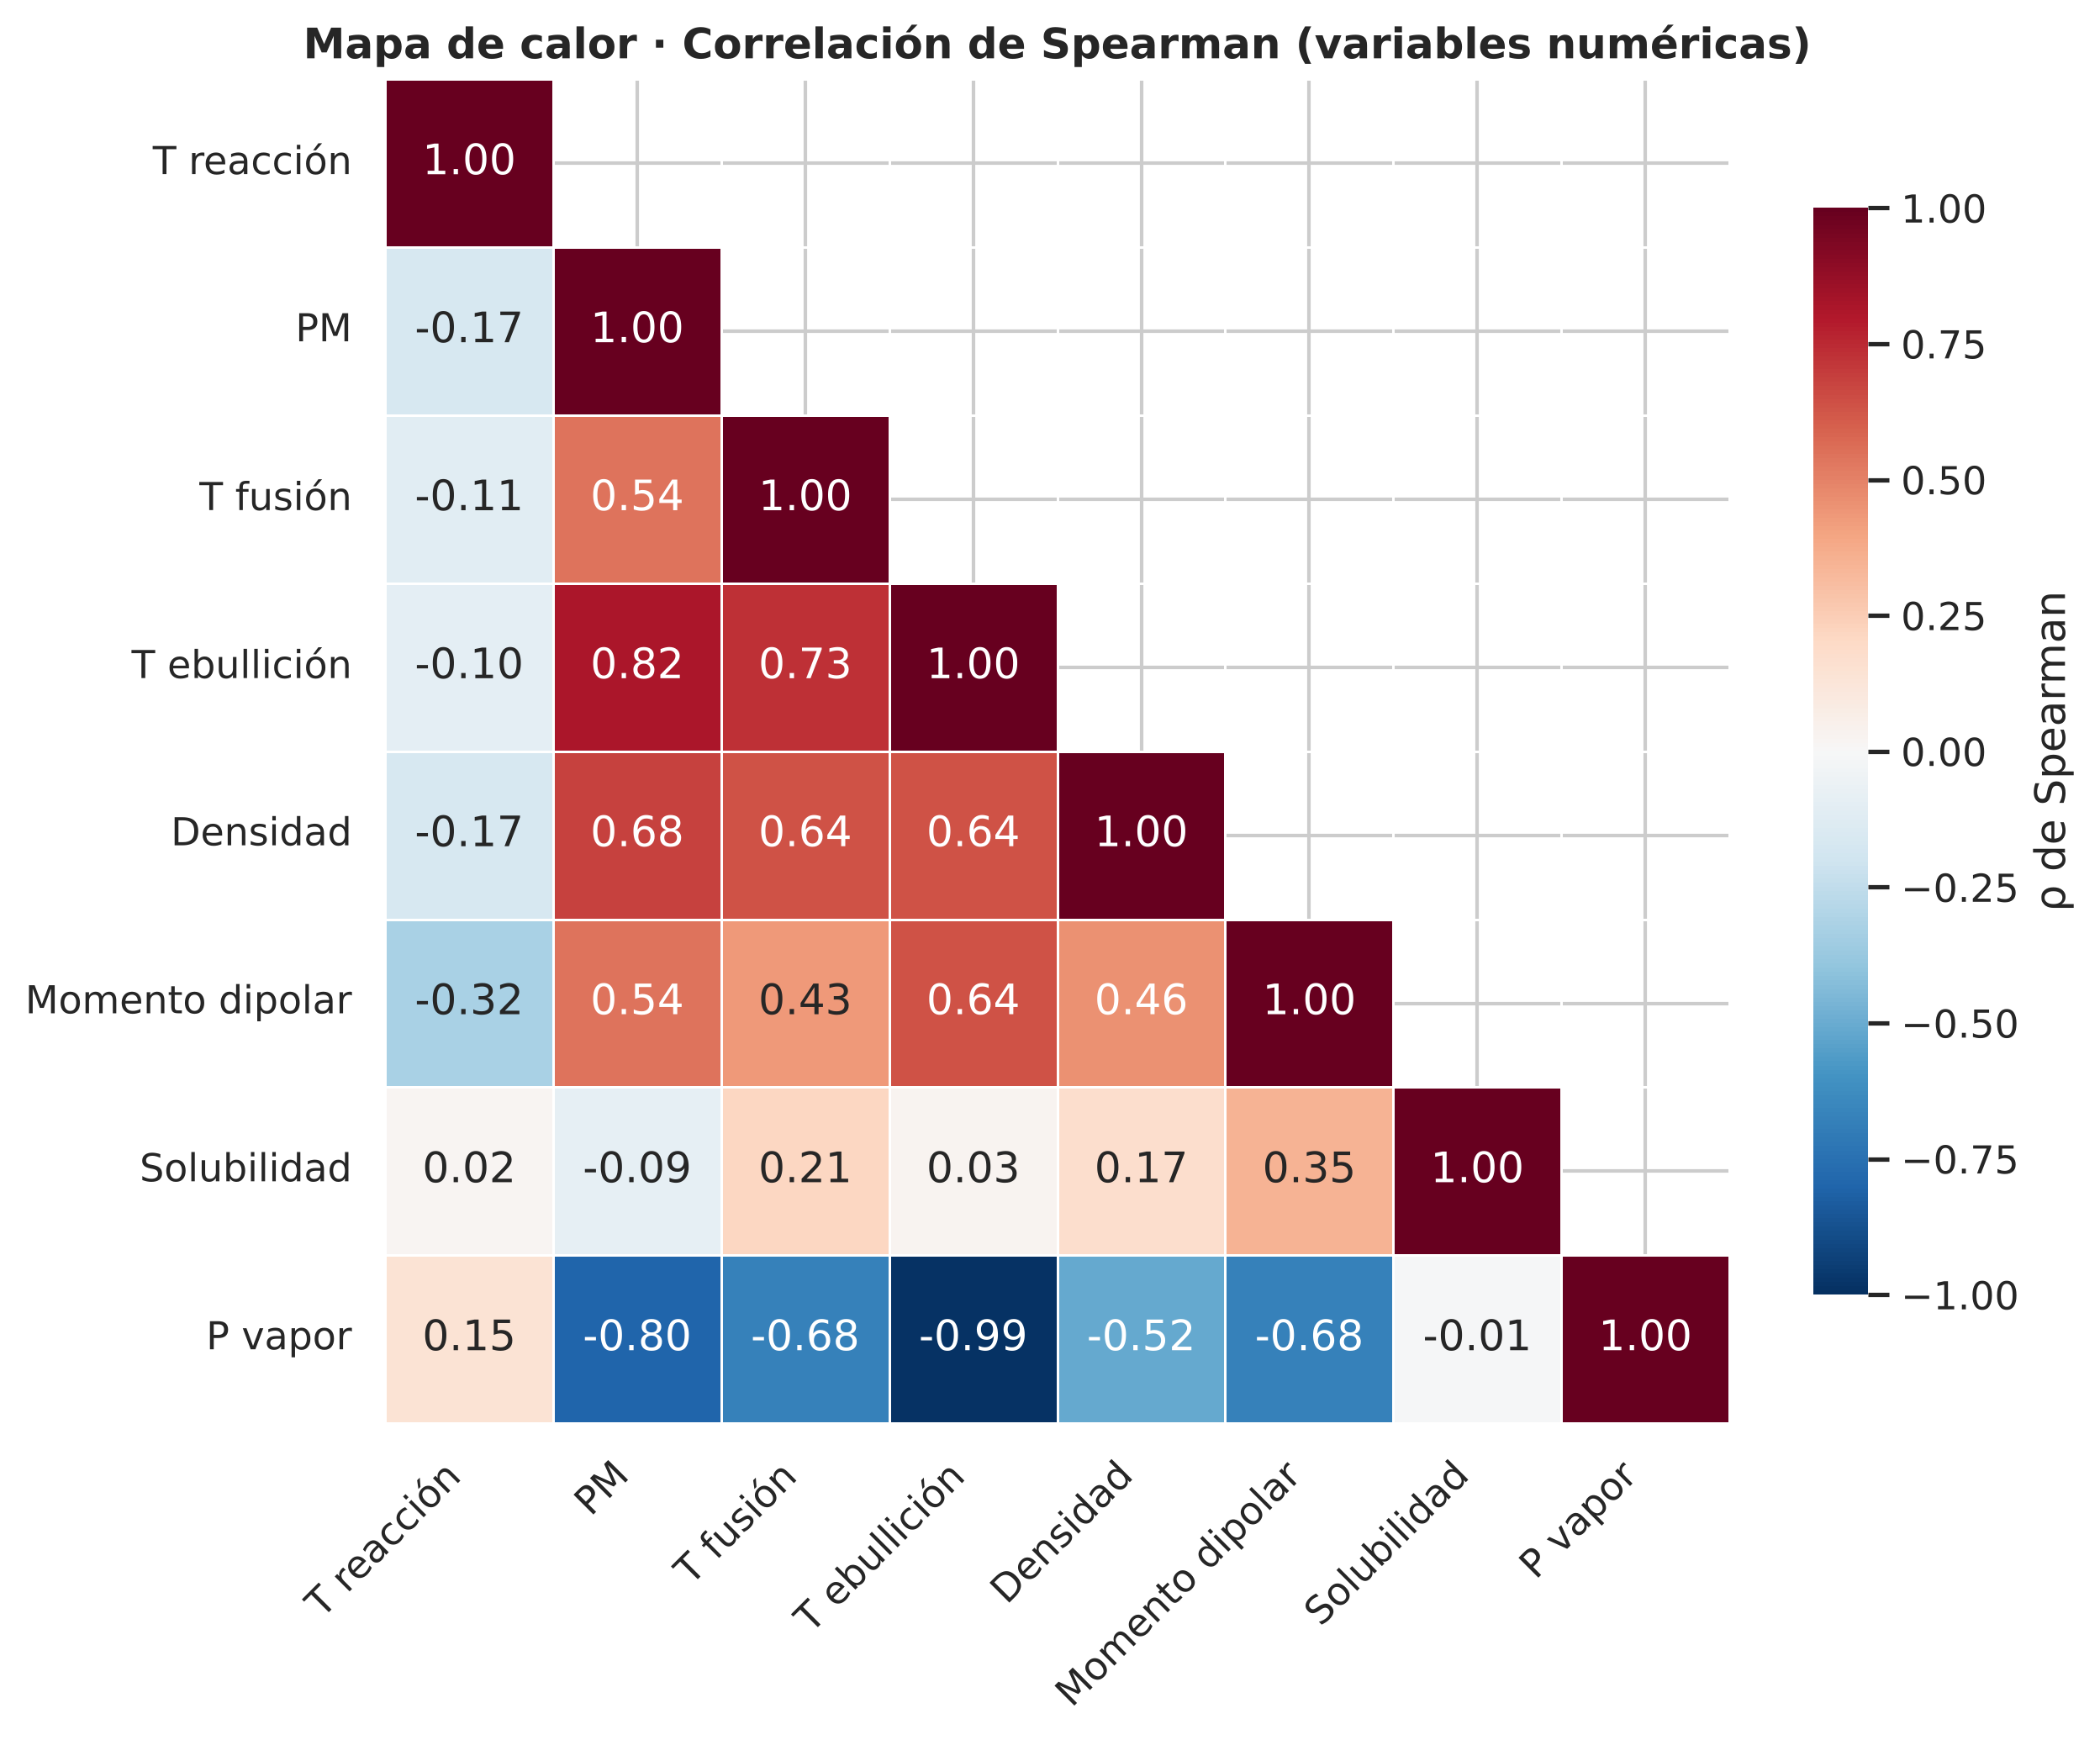
\includegraphics[width=\columnwidth]{02_heatmap_spearman.png}
\caption{Mapa de calor de la correlaci\'on de Spearman entre las variables num\'ericas.}
\label{fig:spearman}
\end{figure}

En el mapa de la $V$ de Cram\'er (figura~\ref{fig:cramer}) hay que separar las asociaciones reales de las redundancias por construcci\'on: $V=0{,}98$ entre sustancia y clase aparece porque cada sustancia pertenece a una sola clase. Las asociaciones reales m\'as altas son familia con tipo de consulta ($V=0{,}76$), cat\'alizador con medio (0,58) y familia con medio (0,53). La sustancia consultada casi no se asocia con ninguna otra variable ($V\leq0{,}22$), as\'i que las condiciones dependen del tipo de transformaci\'on y no de la sustancia que se consulta.

\begin{figure}[!htbp]
\centering
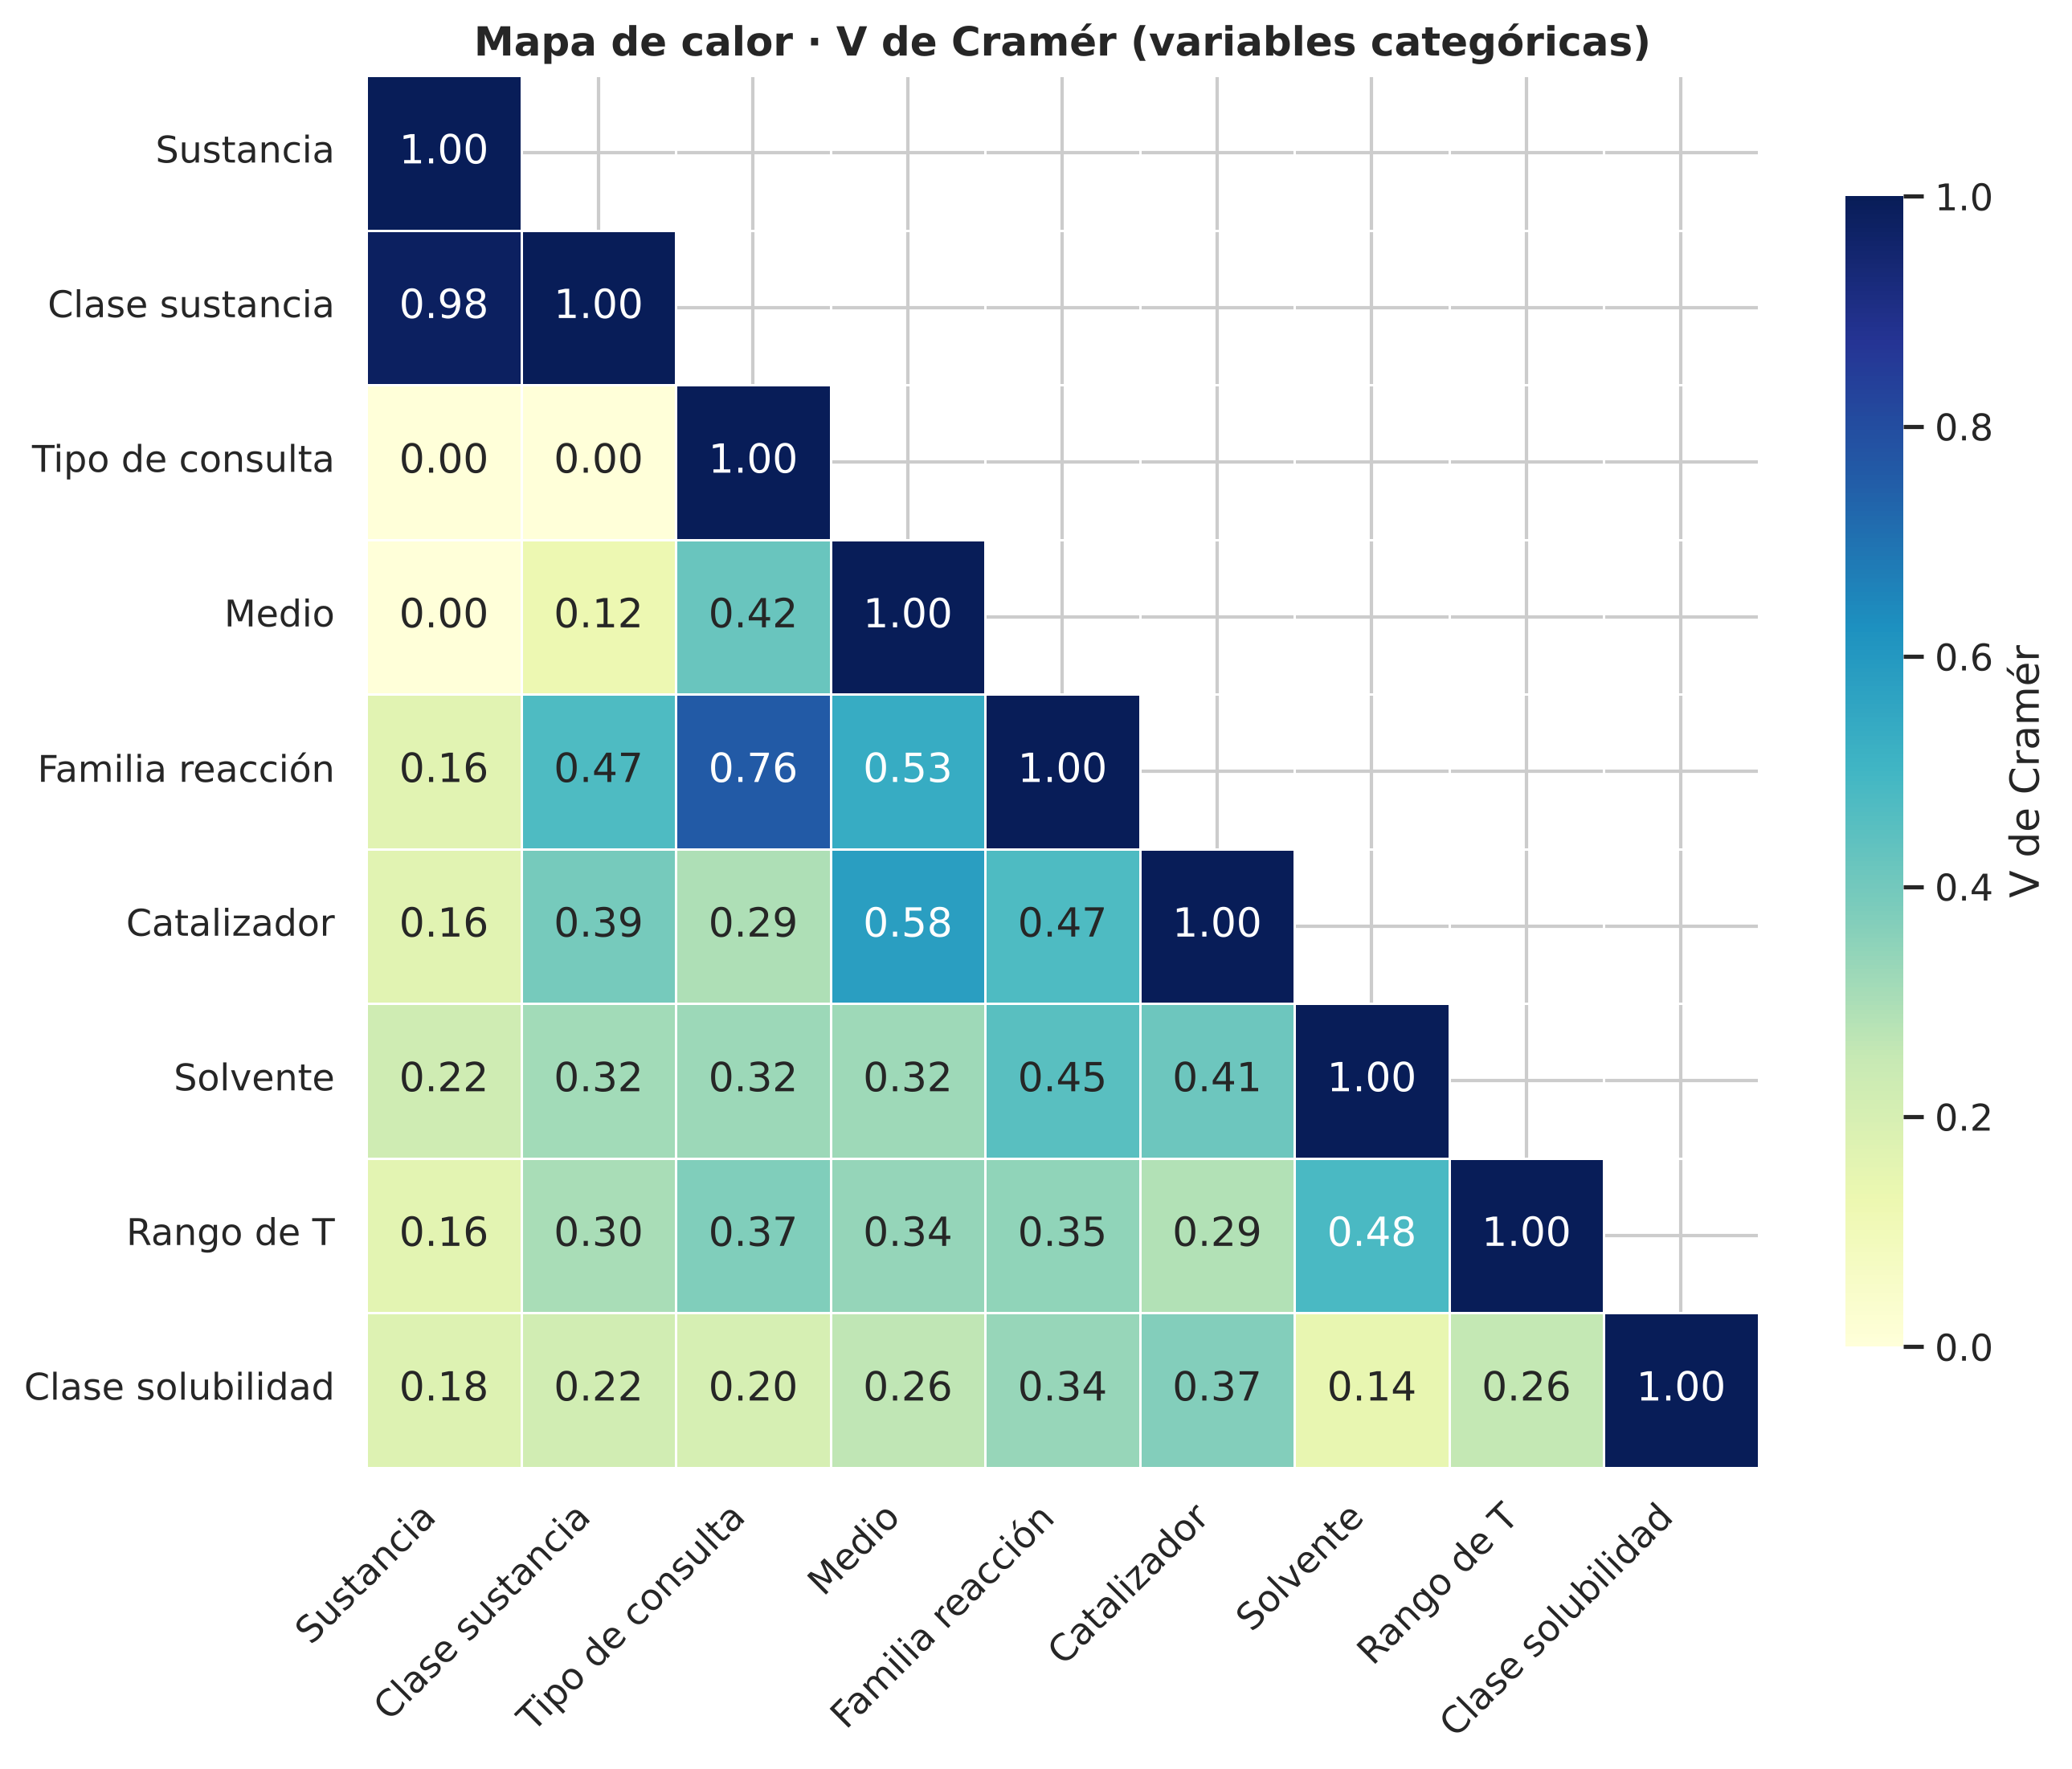
\includegraphics[width=\columnwidth]{03_heatmap_cramer.png}
\caption{Mapa de calor de la $V$ de Cram\'er (corregida) entre las variables categ\'oricas.}
\label{fig:cramer}
\end{figure}

\subsection{Propiedades f\'isicas: tendencia con el peso molecular}
La figura~\ref{fig:pm-teb} confirma H1: el punto de ebullici\'on crece con el PM ($\rho=0{,}82$, $p\approx10^{-45}$, $n=184$), de modo que el PM explica cerca de dos tercios ($\rho^2=0{,}67$) de la variaci\'on. La relaci\'on es curva y la dispersi\'on alrededor de la tendencia se debe a la polaridad: a igual PM, los compuestos con grupos hidroxilo o carbonilo hierven a mayor temperatura que los hidrocarburos por los puentes de hidr\'ogeno y las fuerzas dipolo-dipolo \cite{Clayden2012}. Reacciones y obtenciones se mezclan en la misma nube de puntos, as\'i que la direcci\'on de la consulta no altera la relaci\'on.

\begin{figure}[!htbp]
\centering
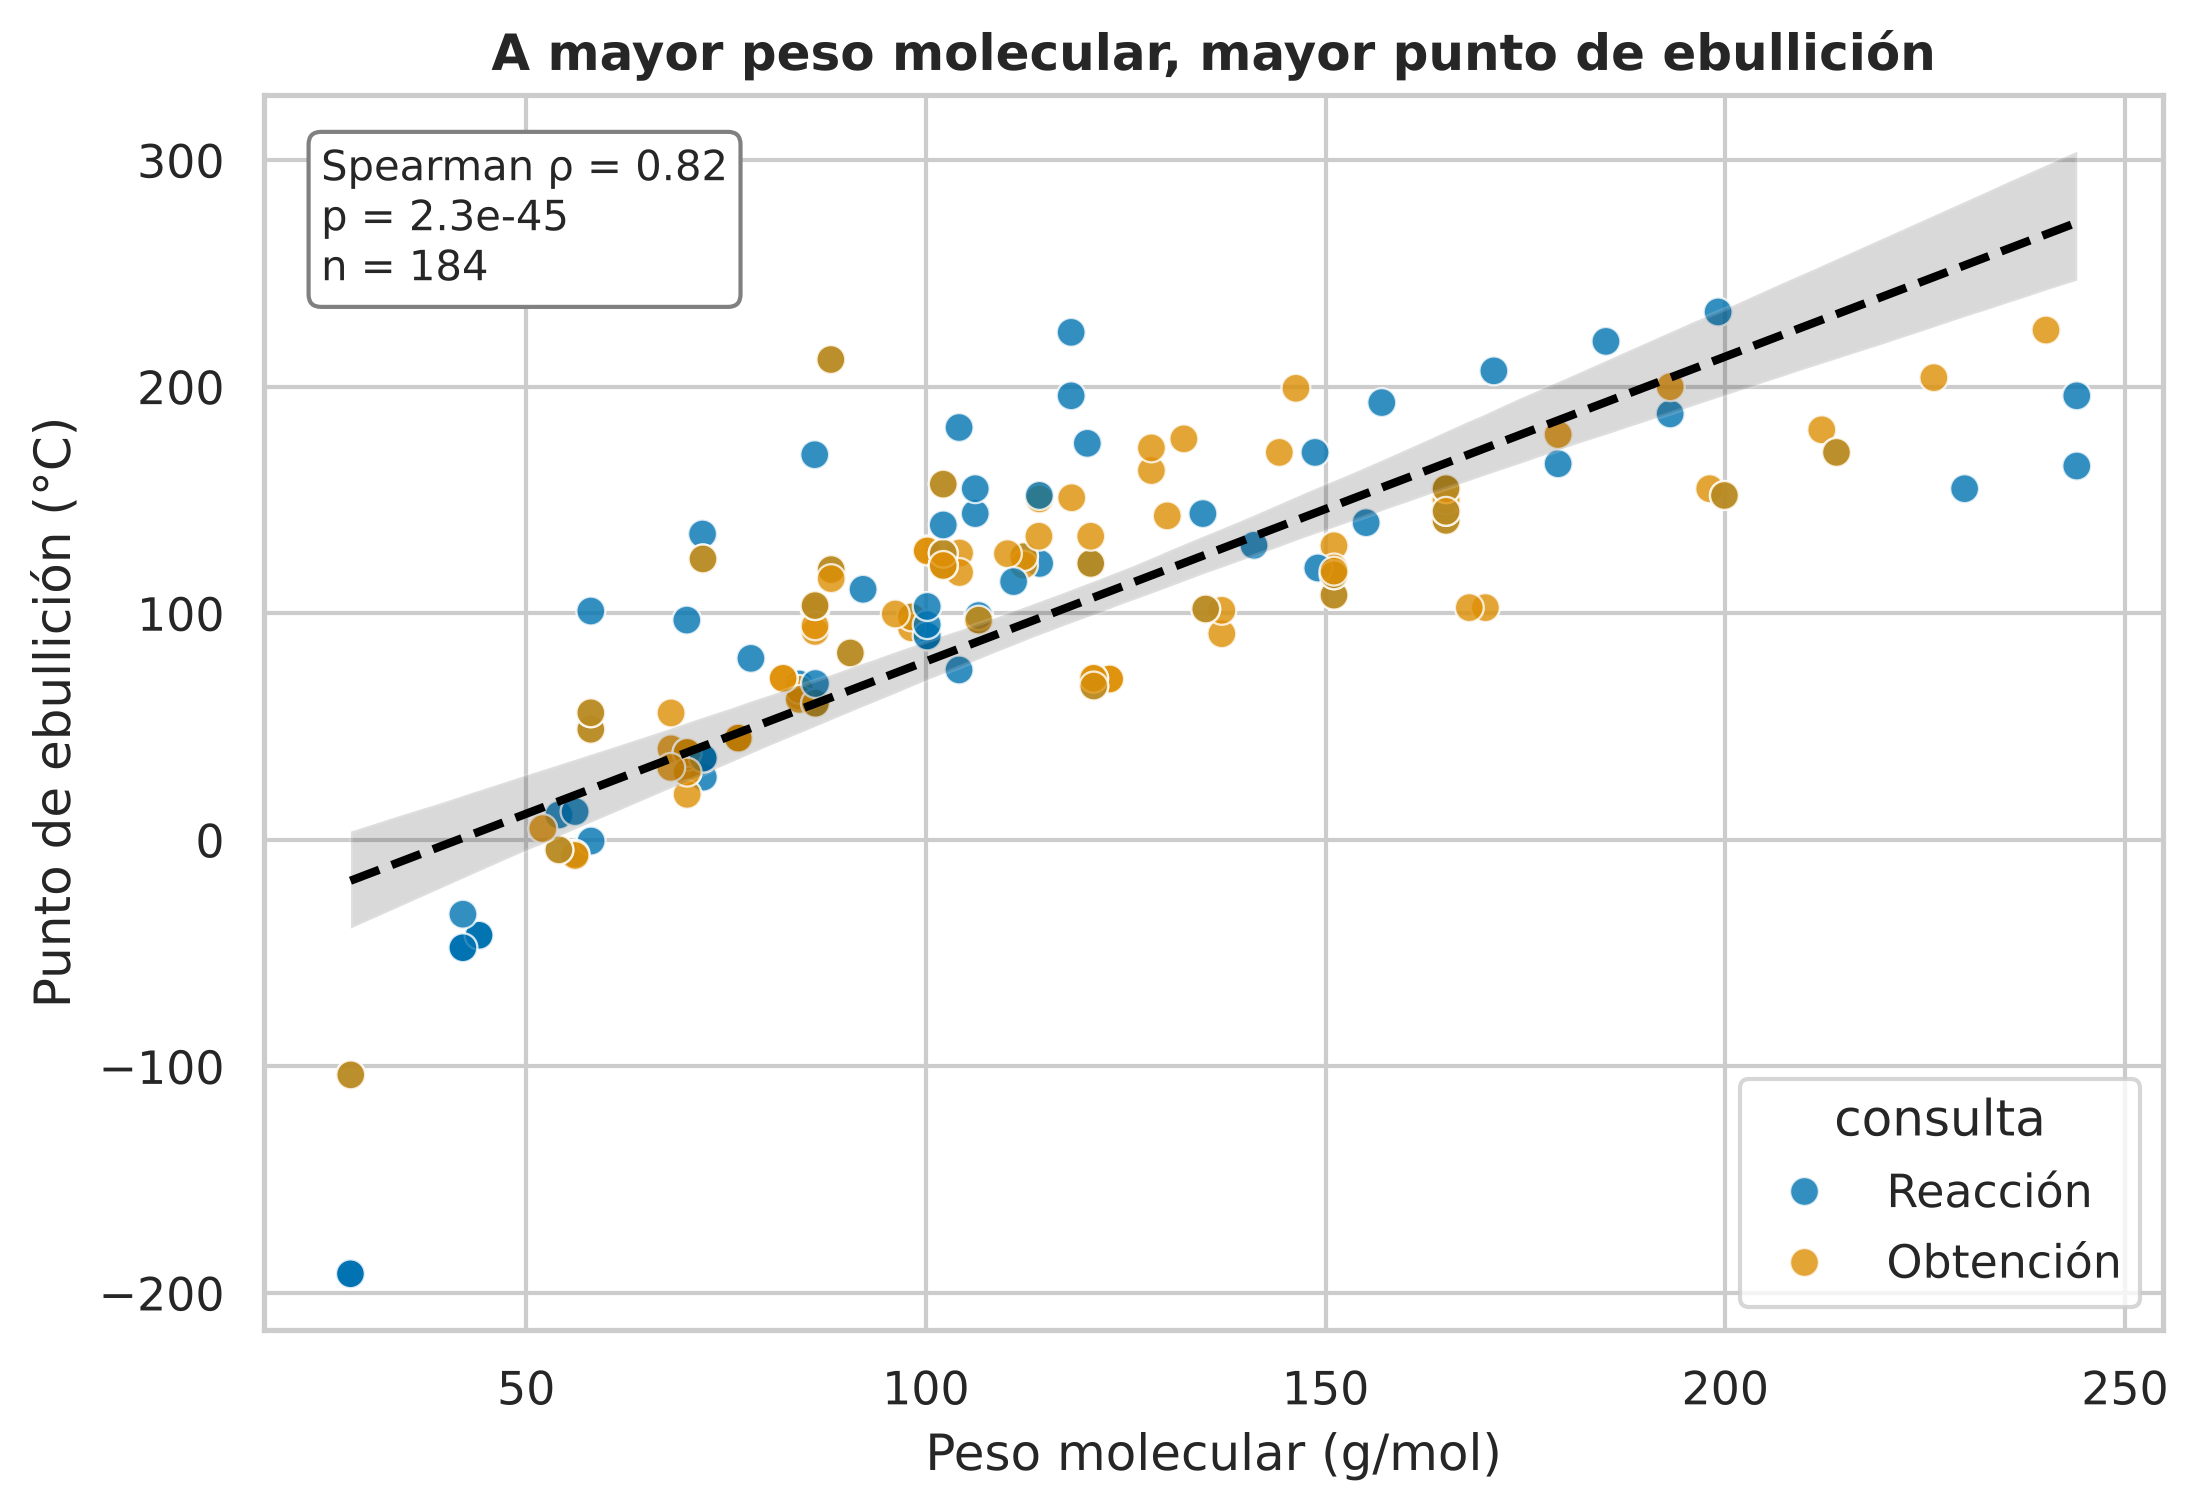
\includegraphics[width=\columnwidth]{05_PM_vs_Teb.png}
\caption{Punto de ebullici\'on frente al peso molecular, con recta de tendencia.}
\label{fig:pm-teb}
\end{figure}

La presi\'on de vapor se comporta de forma opuesta y a\'un m\'as ordenada frente al punto de ebullici\'on (figura~\ref{fig:teb-pvap}): $\rho=-0{,}99$, tal como prev\'e la ecuaci\'on de Clausius-Clapeyron \cite{Atkins2014}. Esto implica que ambas propiedades aportan casi la misma informaci\'on, por lo que en un modelo o en un filtro basta con usar una de las dos. La banda horizontal en la parte superior corresponde a gases cuya presi\'on de vapor se report\'o como 760\,mmHg, un techo de la tabla y no una propiedad real.

\begin{figure}[!htbp]
\centering
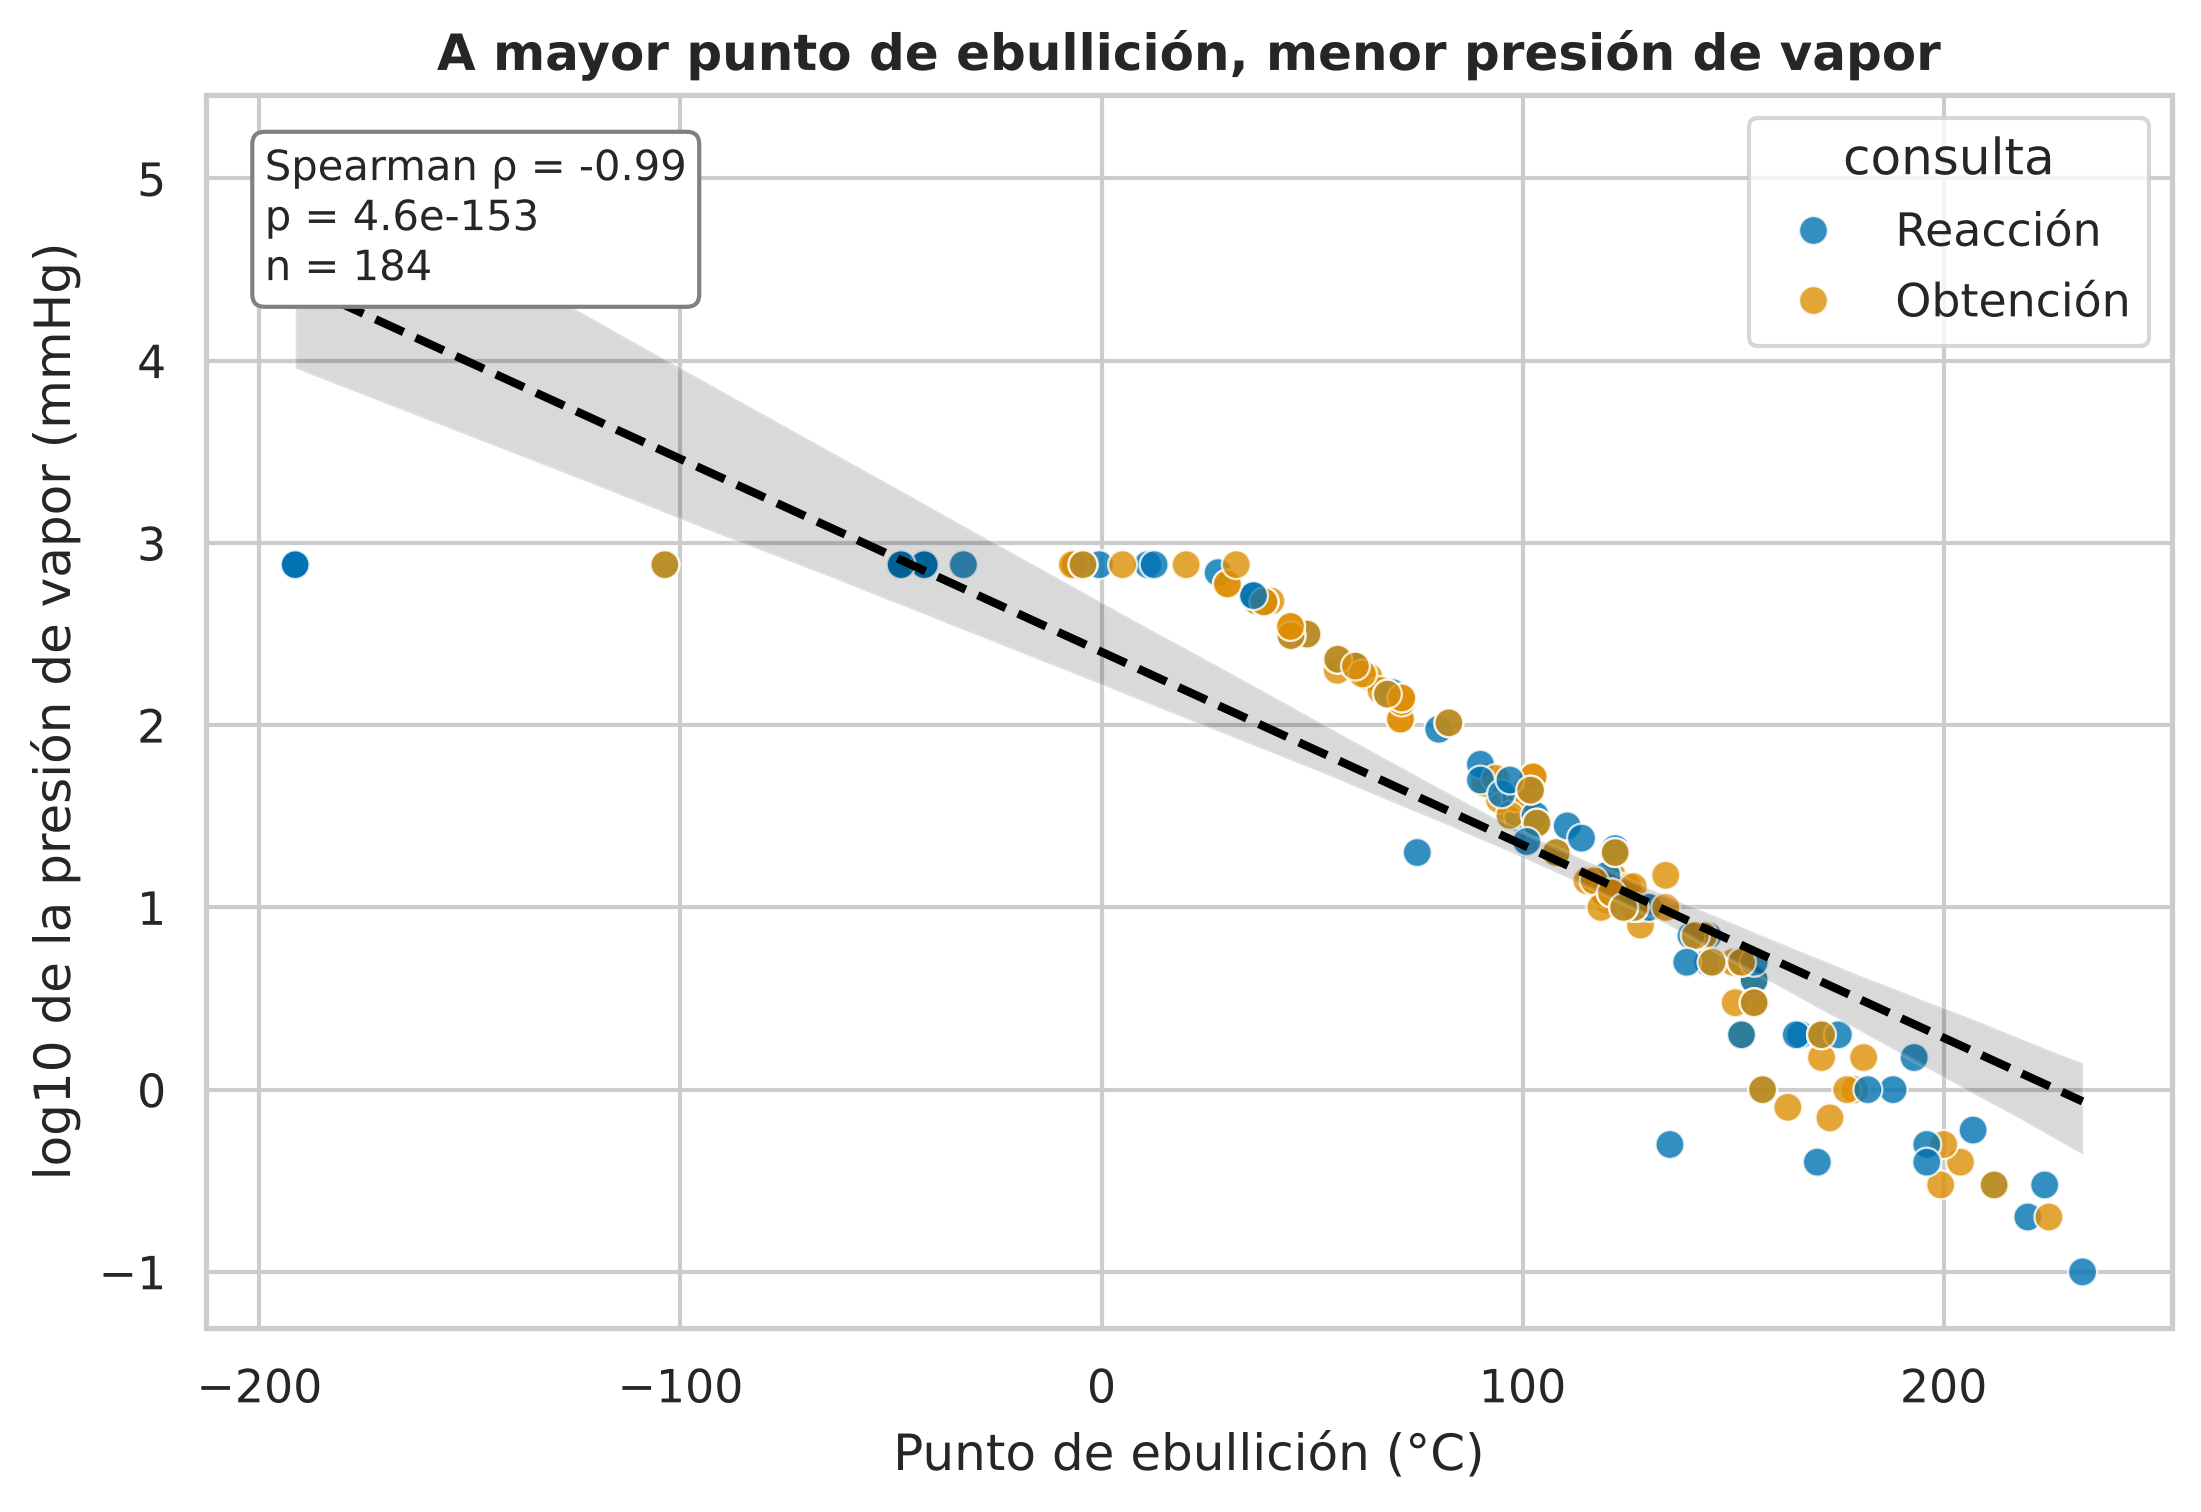
\includegraphics[width=\columnwidth]{07_Teb_vs_Pvap.png}
\caption{Logaritmo de la presi\'on de vapor frente al punto de ebullici\'on.}
\label{fig:teb-pvap}
\end{figure}

La serie de las sustancias consultadas (tabla~\ref{tab:sustancias} y figura~\ref{fig:serie}) muestra la regularidad de una serie hom\'ologa: el punto de ebullici\'on de los alcanos lineales sube de 36,1 (pentano) a 69,0 (hexano), 98,4 (heptano) y 125,7\,\textdegree C (octano), es decir, unos 33, 29 y 27\,\textdegree C por cada $-\mathrm{CH_2}-$. El isopentano, ramificado, hierve m\'as bajo (27,7\,\textdegree C) que el pentano (36,1\,\textdegree C) con el mismo PM. Los alquenos hierven casi igual que el alcano de igual n\'umero de carbonos (pent-2-eno 36,9\,\textdegree C y hex-1-eno 63,5\,\textdegree C), porque el doble enlace cambia poco la polaridad, y los cicloalquenos de bajo PM (ciclopropeno $-36$\,\textdegree C y ciclobuteno 2\,\textdegree C) son gases o casi gases a temperatura ambiente.

\begin{table*}[!t]
	\centering
	\footnotesize
	\begin{tabular}{|l|c|c|c|c|c|c|c|}
		\hline
		\textbf{Sustancia} & \textbf{PM (g/mol)} & \textbf{$T_f$ (\textdegree C)} & \textbf{$T_{eb}$ (\textdegree C)} & \textbf{Densidad (g/cm$^3$)} & \textbf{$\mu$ (D)} & \textbf{Solubilidad (g/L)} & \textbf{$P_{vap}$ (mmHg)} \\
		\hline
		Pentano & 72,15 & $-130{,}0$ & 36,1 & 0,626 & 0,00 & 0,04 & 514 \\
		Isopentano & 72,15 & $-159{,}9$ & 27,7 & 0,620 & 0,13 & 0,048 & 687 \\
		Hexano & 86,18 & $-95{,}3$ & 69,0 & 0,659 & 0,00 & 0,013 & 151 \\
		Heptano & 100,21 & $-90{,}6$ & 98,4 & 0,684 & 0,00 & 0,003 & 40 \\
		Octano & 114,23 & $-56{,}8$ & 125,7 & 0,703 & 0,00 & 0,001 & 11 \\
		Pent-2-eno & 70,13 & $-151{,}4$ & 36,9 & 0,650 & 0,50 & 0,203 & 480 \\
		2-Metilpent-2-eno & 84,16 & $-135{,}1$ & 67,3 & 0,669 & 0,30 & 0,078 & 143 \\
		Hex-1-eno & 84,16 & $-139{,}8$ & 63,5 & 0,673 & 0,30 & 0,050 & 184 \\
		Ciclopropeno & 40,06 & $-87{,}0$ & $-36{,}0$ & 0,688 & 0,45 & 0,28 & 760 \\
		Ciclobuteno & 54,09 & $-98{,}0$ & 2,0 & 0,733 & 0,53 & 0,42 & 760 \\
		\hline
	\end{tabular}
	\captionsetup{width=\textwidth, justification=justified}
	\caption{Propiedades fisicoqu\'imicas de las diez sustancias consultadas.}
	\label{tab:sustancias}
\end{table*}

\begin{figure}[!htbp]
\centering
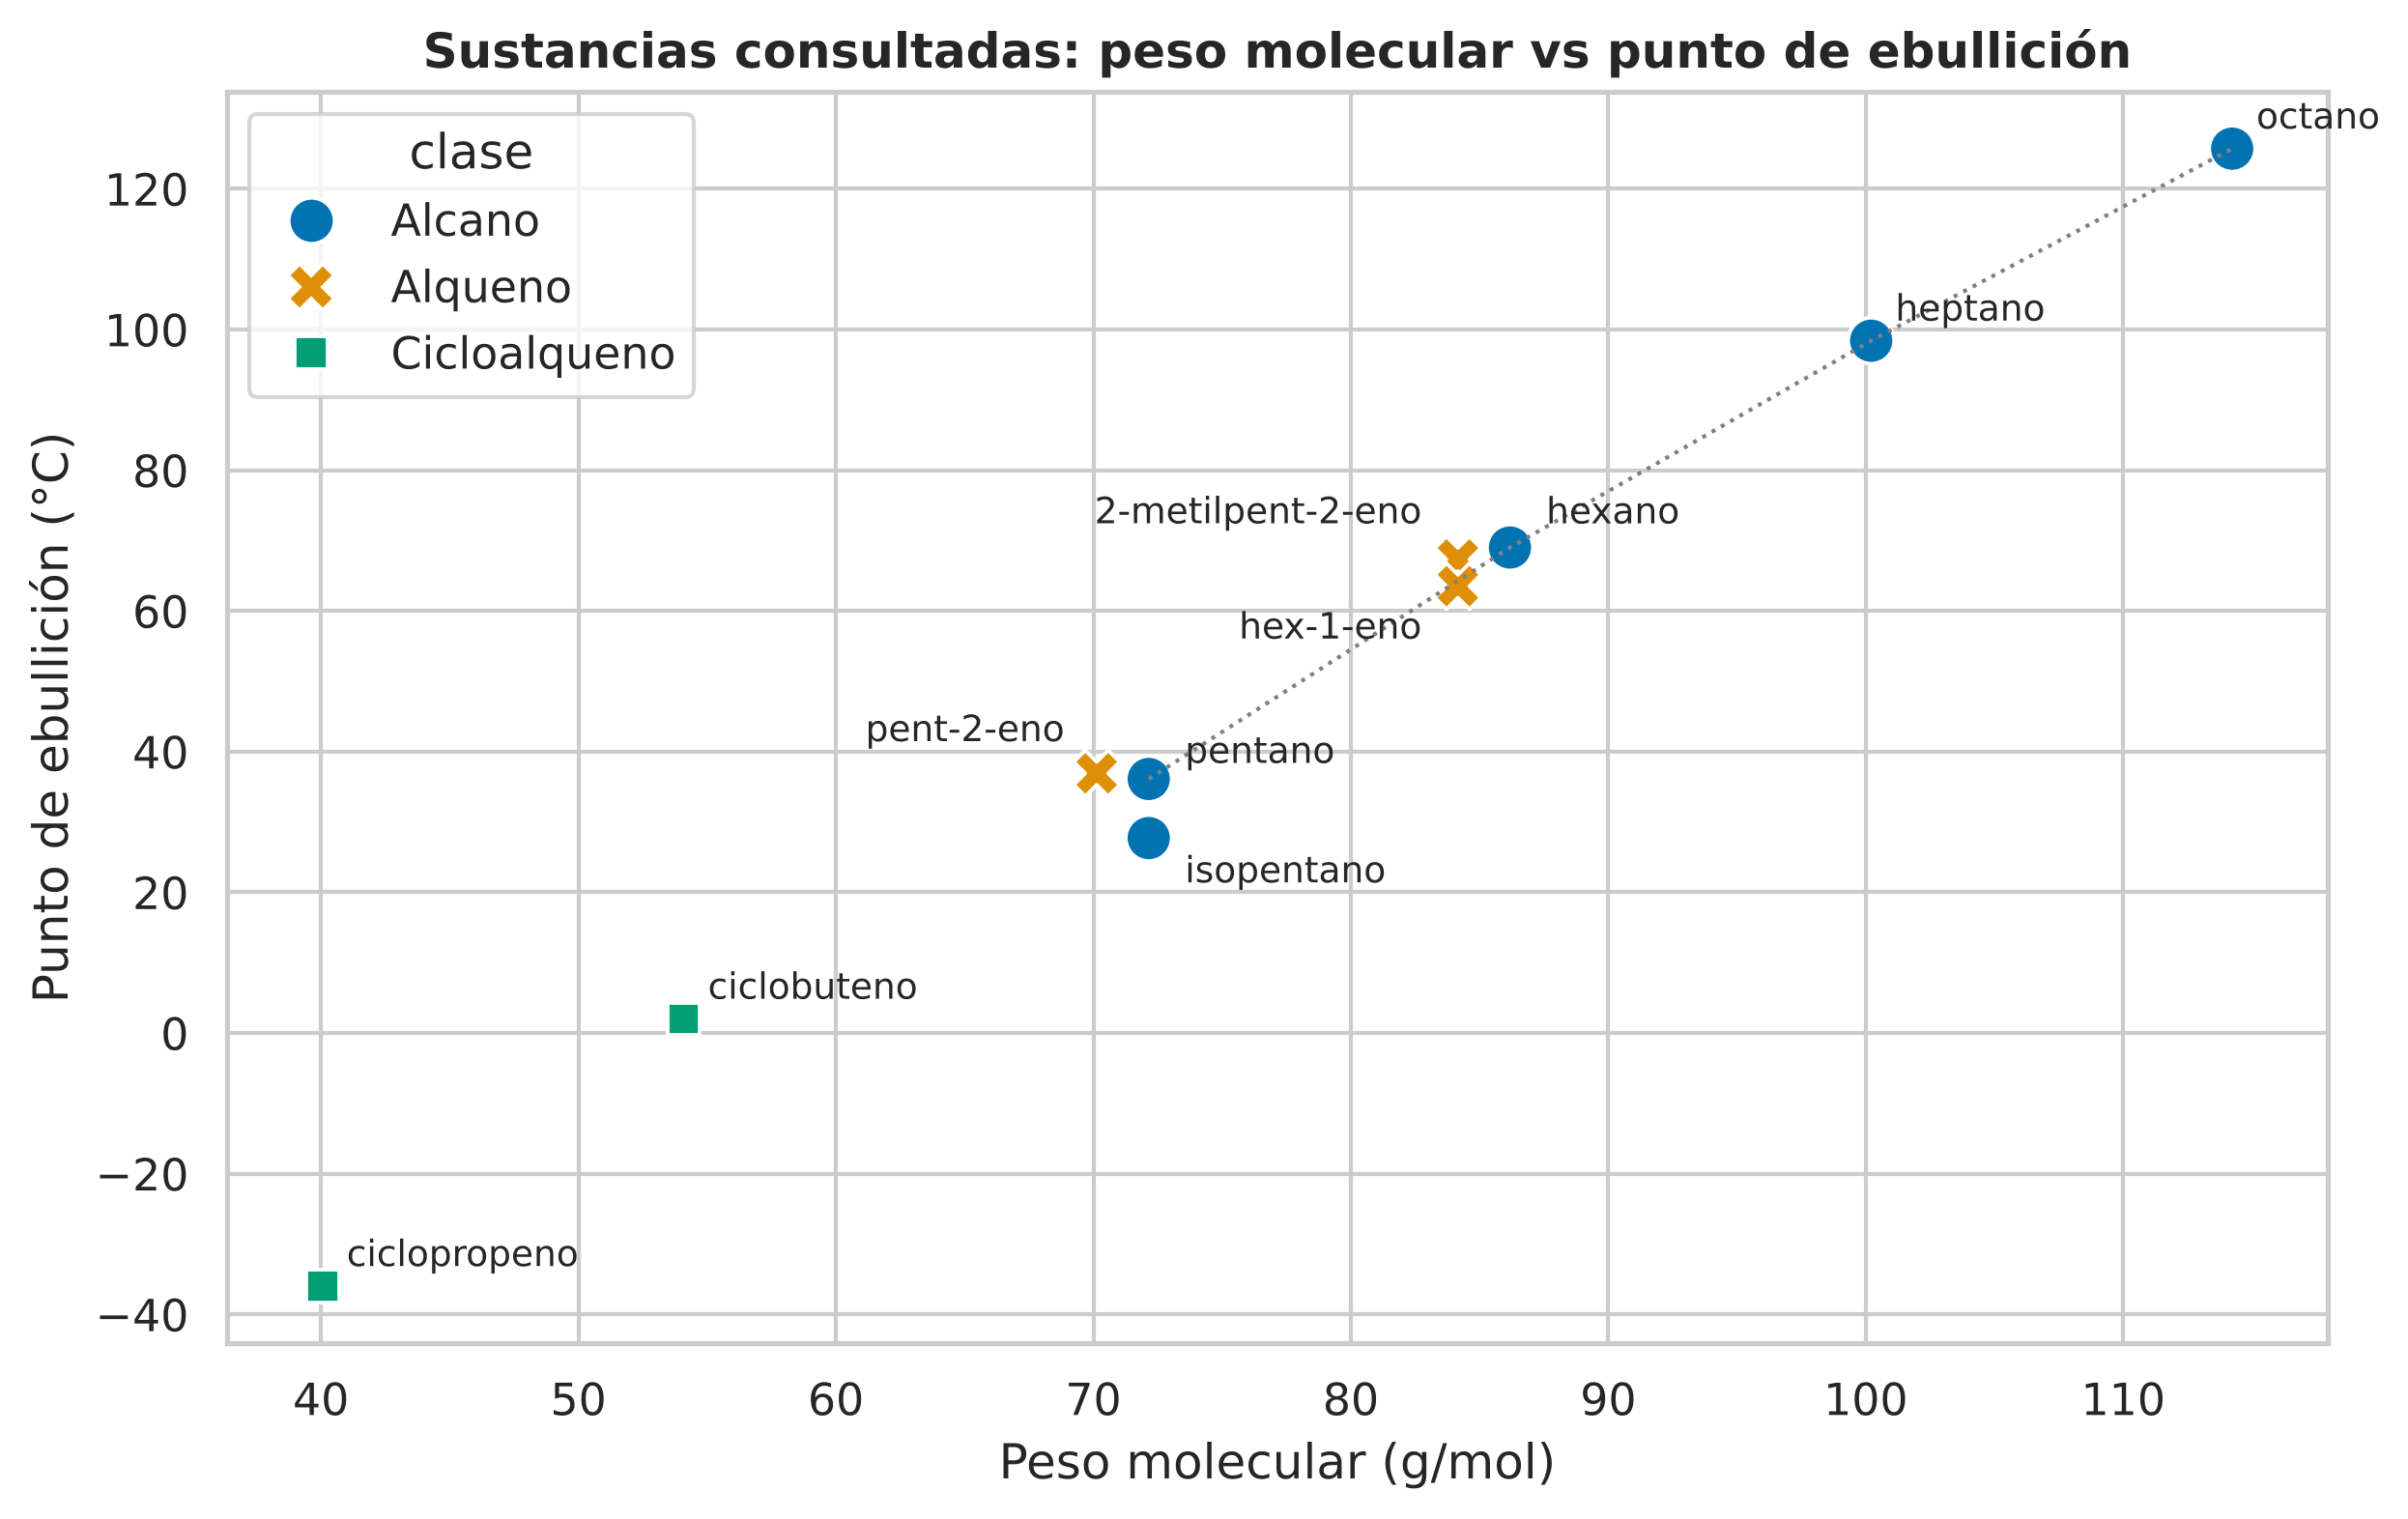
\includegraphics[width=\columnwidth]{08_serie_sustancias_consultadas.png}
\caption{Peso molecular y punto de ebullici\'on de las sustancias consultadas.}
\label{fig:serie}
\end{figure}

\subsection{Condiciones de reacci\'on: probabilidad condicional}
La figura~\ref{fig:prob-medio} muestra la probabilidad del medio dado la familia de reacci\'on, $P(\text{medio}\mid\text{familia})$, que se compara con la probabilidad global de cada medio. Los patrones coinciden con los mecanismos: la eliminaci\'on ocurre en medio b\'asico con probabilidad 0,59 (2,7 veces la global, 0,22), de acuerdo con el mecanismo E2 con bases fuertes; la sustituci\'on es apolar con probabilidad 0,79, propia de la halogenaci\'on radicalaria con luz ultravioleta; la oxidaci\'on es neutra con 0,83 (combusti\'on, epoxidaci\'on y dihidroxilaci\'on); y la isomerizaci\'on es \'acida con 0,86, ya que se cataliza con \'acidos de Lewis o de Br\o nsted. Con el catalizador pasa lo mismo (figura~\ref{fig:prob-cat}): la sustituci\'on usa catalizador radicalario en 79\,\% de los casos, la reducci\'on usa metal soportado en 59\,\%, y la oxidaci\'on (77\,\%) y la eliminaci\'on (61\,\%) se hacen con frecuencia sin catalizador. Estos resultados confirman H2. Debe tenerse presente que en isomerizaci\'on ($n=7$) y ciclaci\'on ($n=9$) los porcentajes cambian mucho con un solo registro, por lo que se leen como tendencias.

\begin{figure*}[!t]
\centering
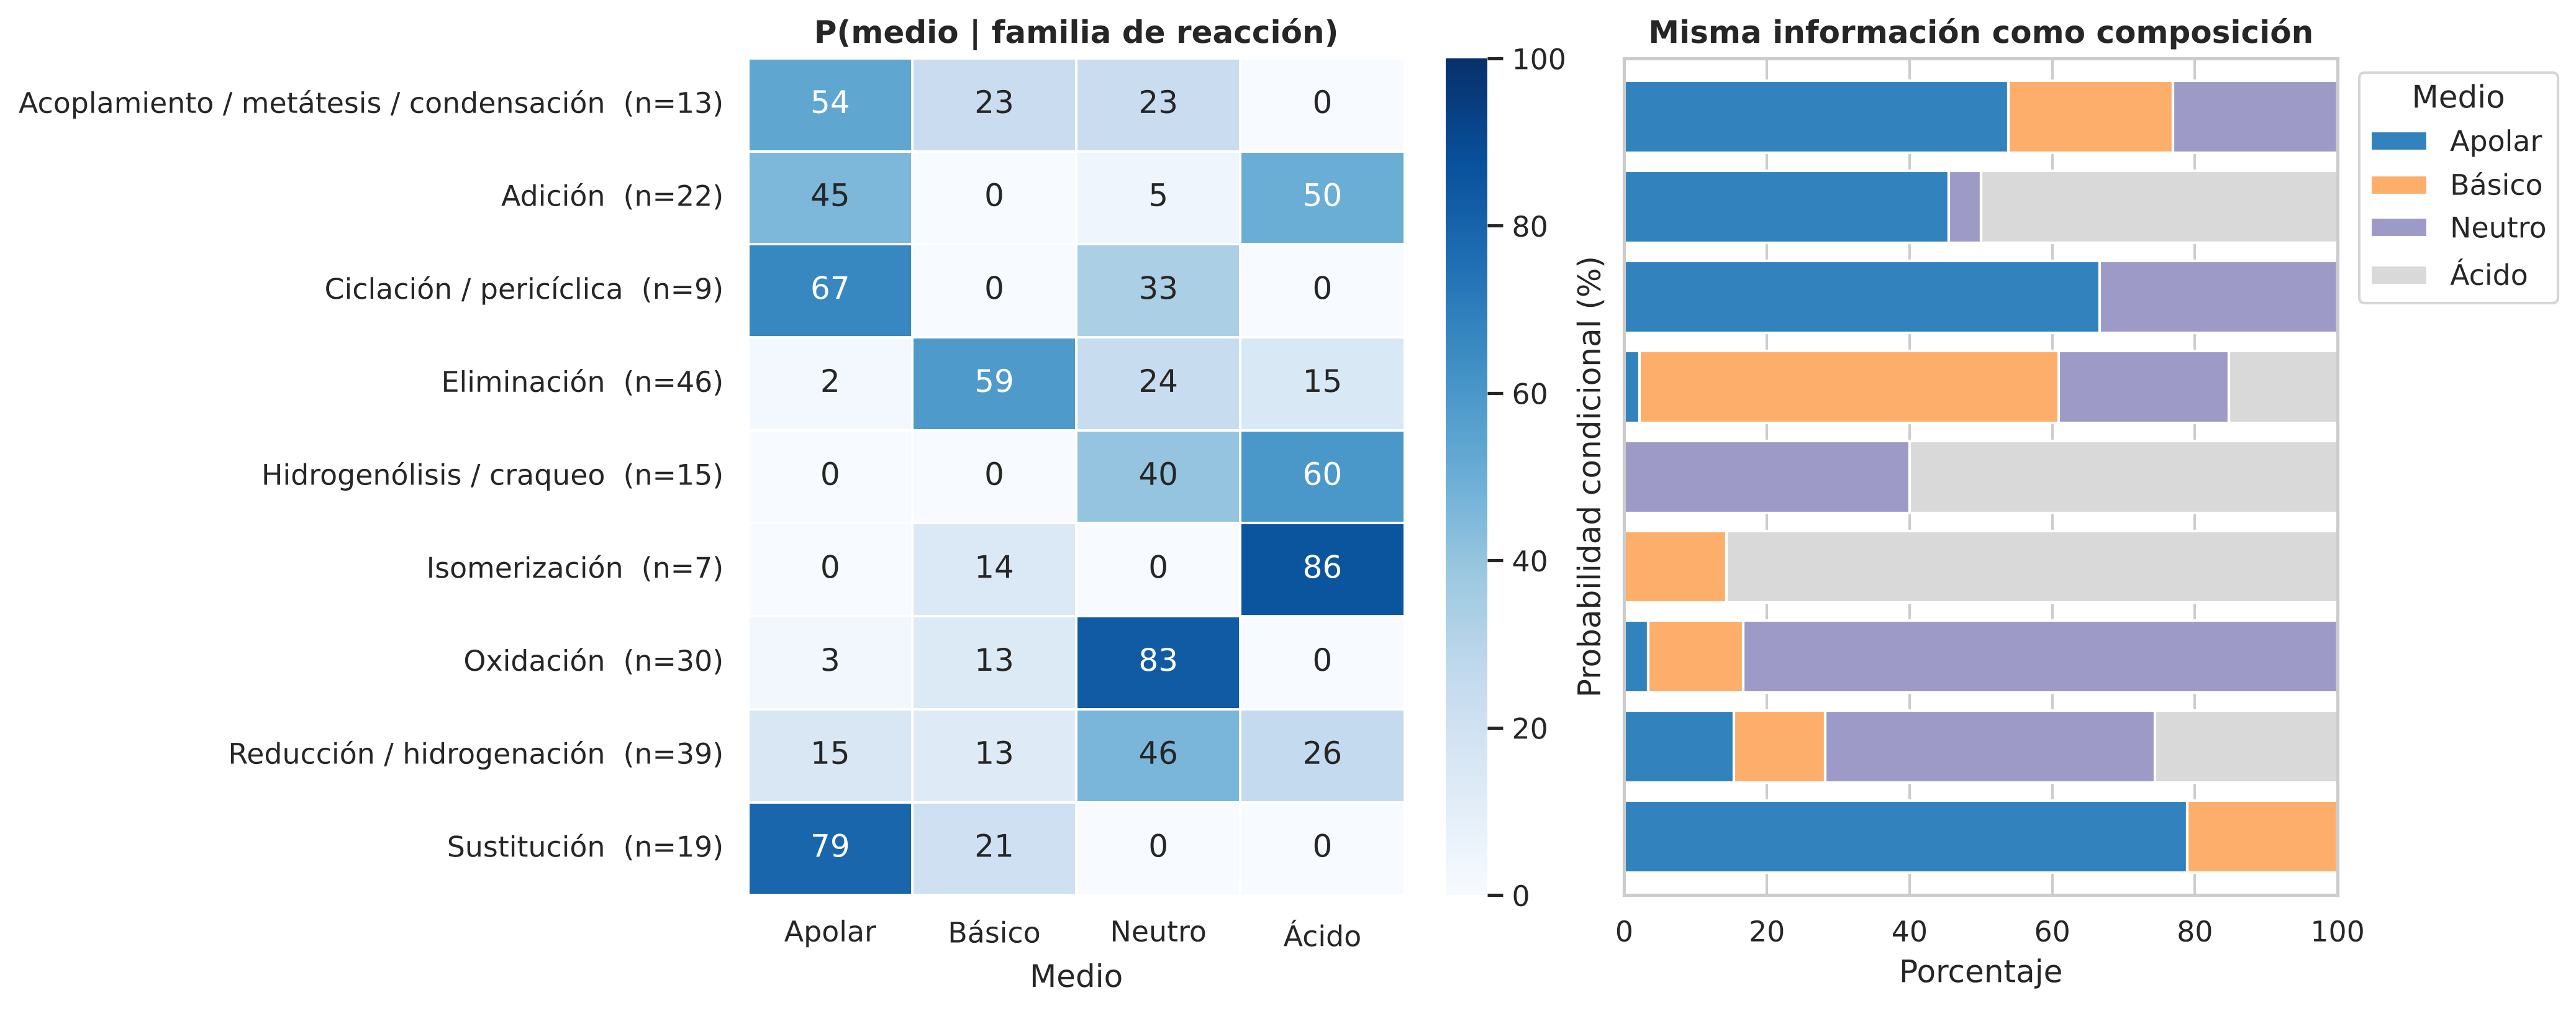
\includegraphics[width=0.92\textwidth]{10_prob_familia_medio.png}
\caption{Probabilidad condicional del medio de reacci\'on seg\'un la familia de reacci\'on (izquierda) y su composici\'on porcentual (derecha).}
\label{fig:prob-medio}
\end{figure*}

\begin{figure*}[!t]
\centering
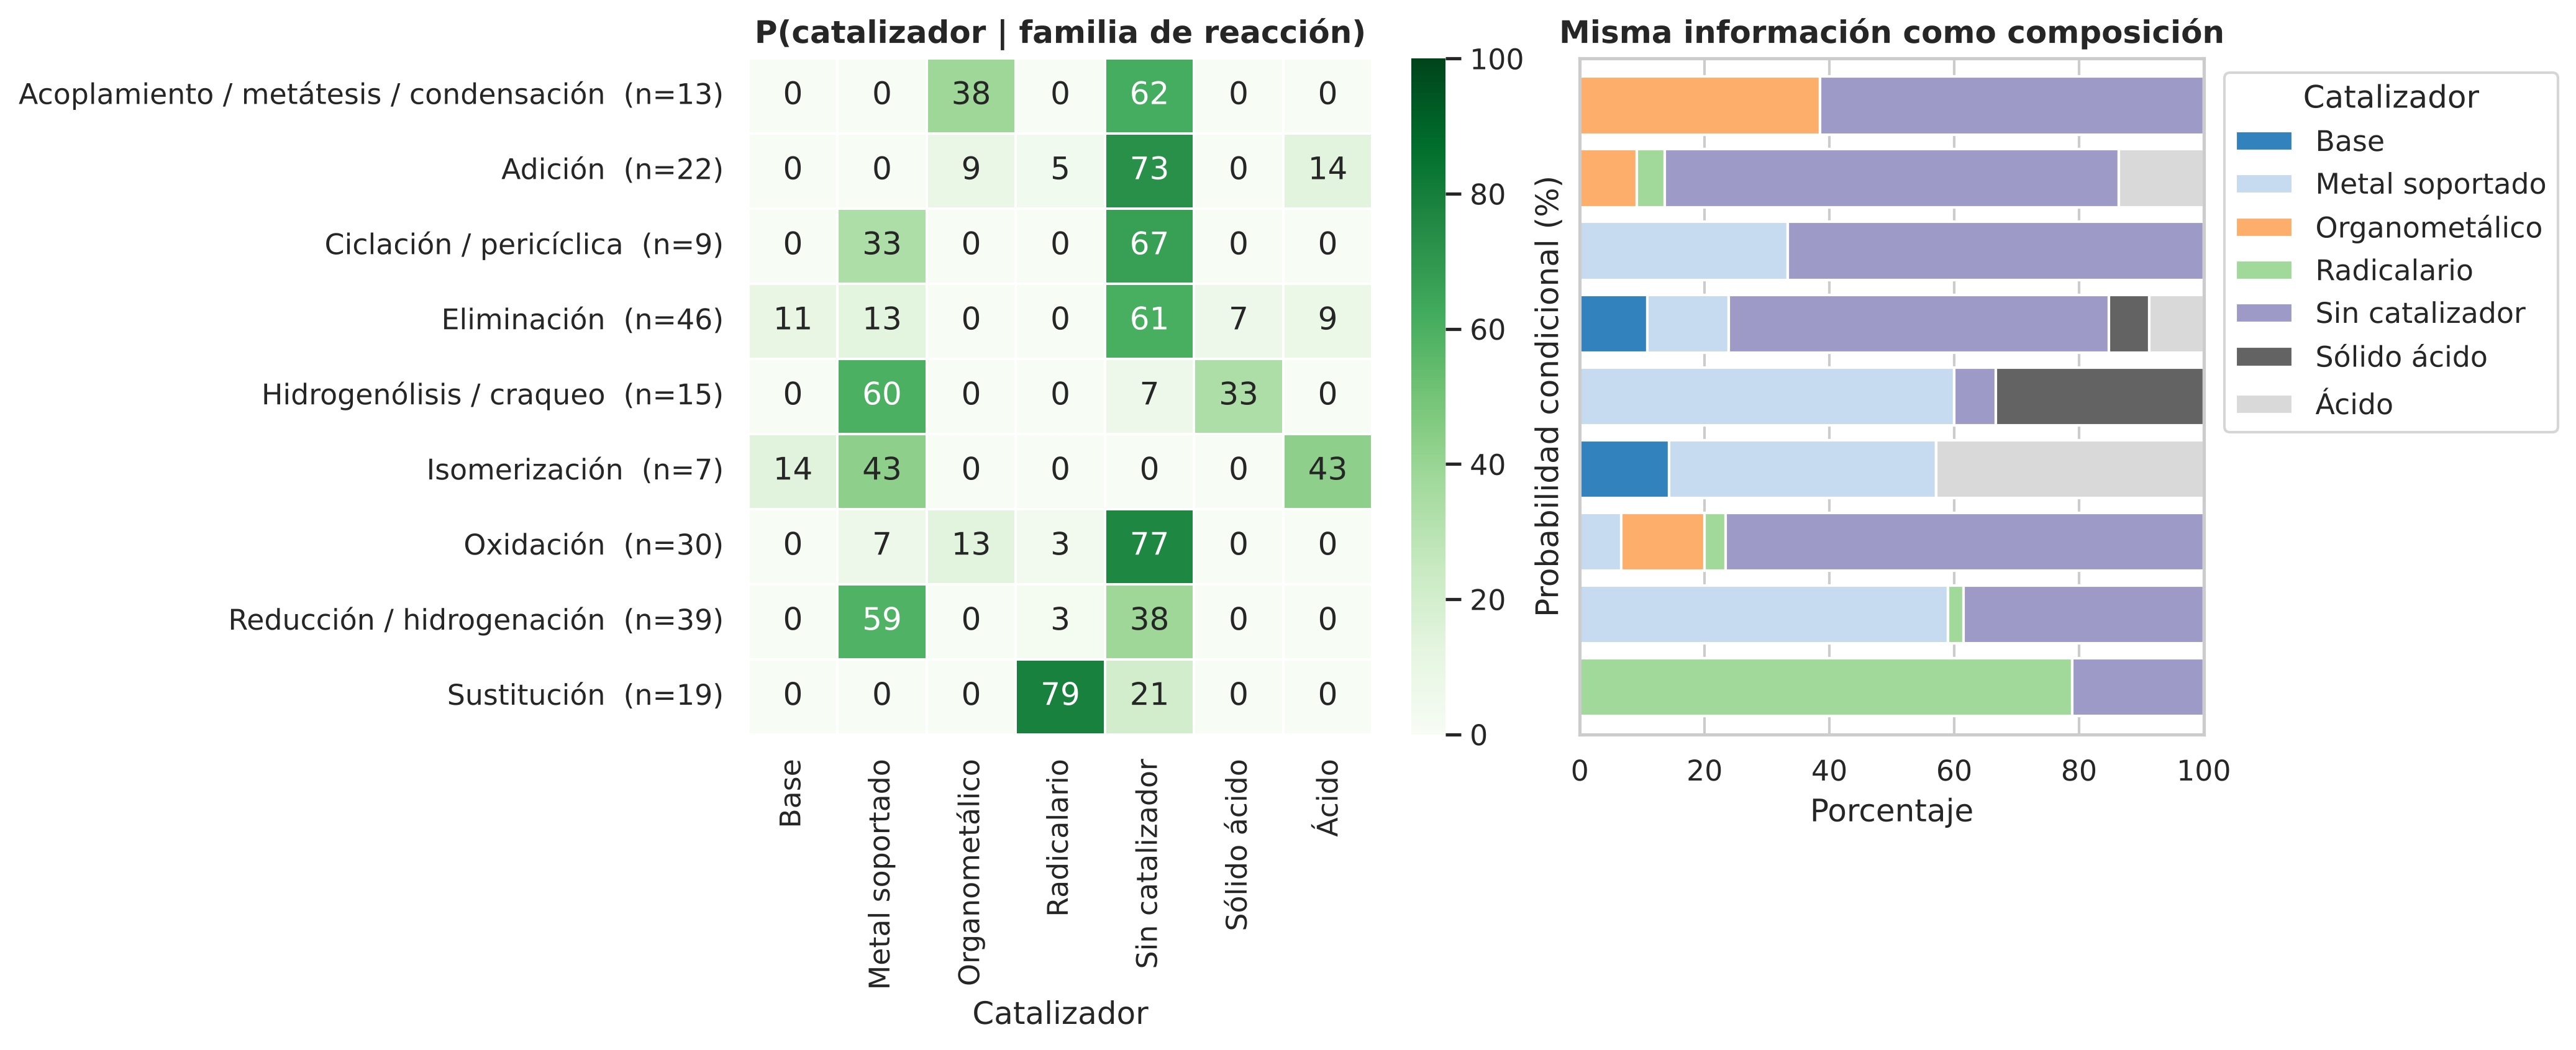
\includegraphics[width=0.92\textwidth]{11_prob_familia_catalizador.png}
\caption{Probabilidad condicional de la categor\'ia de catalizador seg\'un la familia de reacci\'on.}
\label{fig:prob-cat}
\end{figure*}

\subsection{Temperatura de reacci\'on}
La temperatura se agrupa en dos reg\'imenes (figura~\ref{fig:box-t}). La adici\'on, la reducci\'on, la isomerizaci\'on, el acoplamiento y la sustituci\'on tienen medianas entre 25 y 65\,\textdegree C, mientras que la hidrogen\'olisis y el craqueo tienen la mediana m\'as alta (300\,\textdegree C, con un rango de 78 a 750\,\textdegree C), seguidos por la eliminaci\'on (115\,\textdegree C). La oxidaci\'on es un caso especial porque su distribuci\'on es bimodal: mezcla oxidaciones suaves (epoxidaci\'on, ozon\'olisis a $-78$\,\textdegree C) con combustiones a 600--800\,\textdegree C, de modo que su mediana (25\,\textdegree C) no la resume bien. La diferencia entre familias es significativa y de efecto grande (Kruskal-Wallis, $H=49{,}3$, $\varepsilon^2=0{,}22$), con lo que se confirma H3 para la familia; para el catalizador el efecto es mediano ($\varepsilon^2=0{,}08$) y para el solvente es muy grande ($\varepsilon^2=0{,}49$), pero esto \'ultimo no es causal: las reacciones t\'ermicas en fase gas, que son las de mayor temperatura, simplemente no usan solvente.

\begin{figure}[!htbp]
\centering
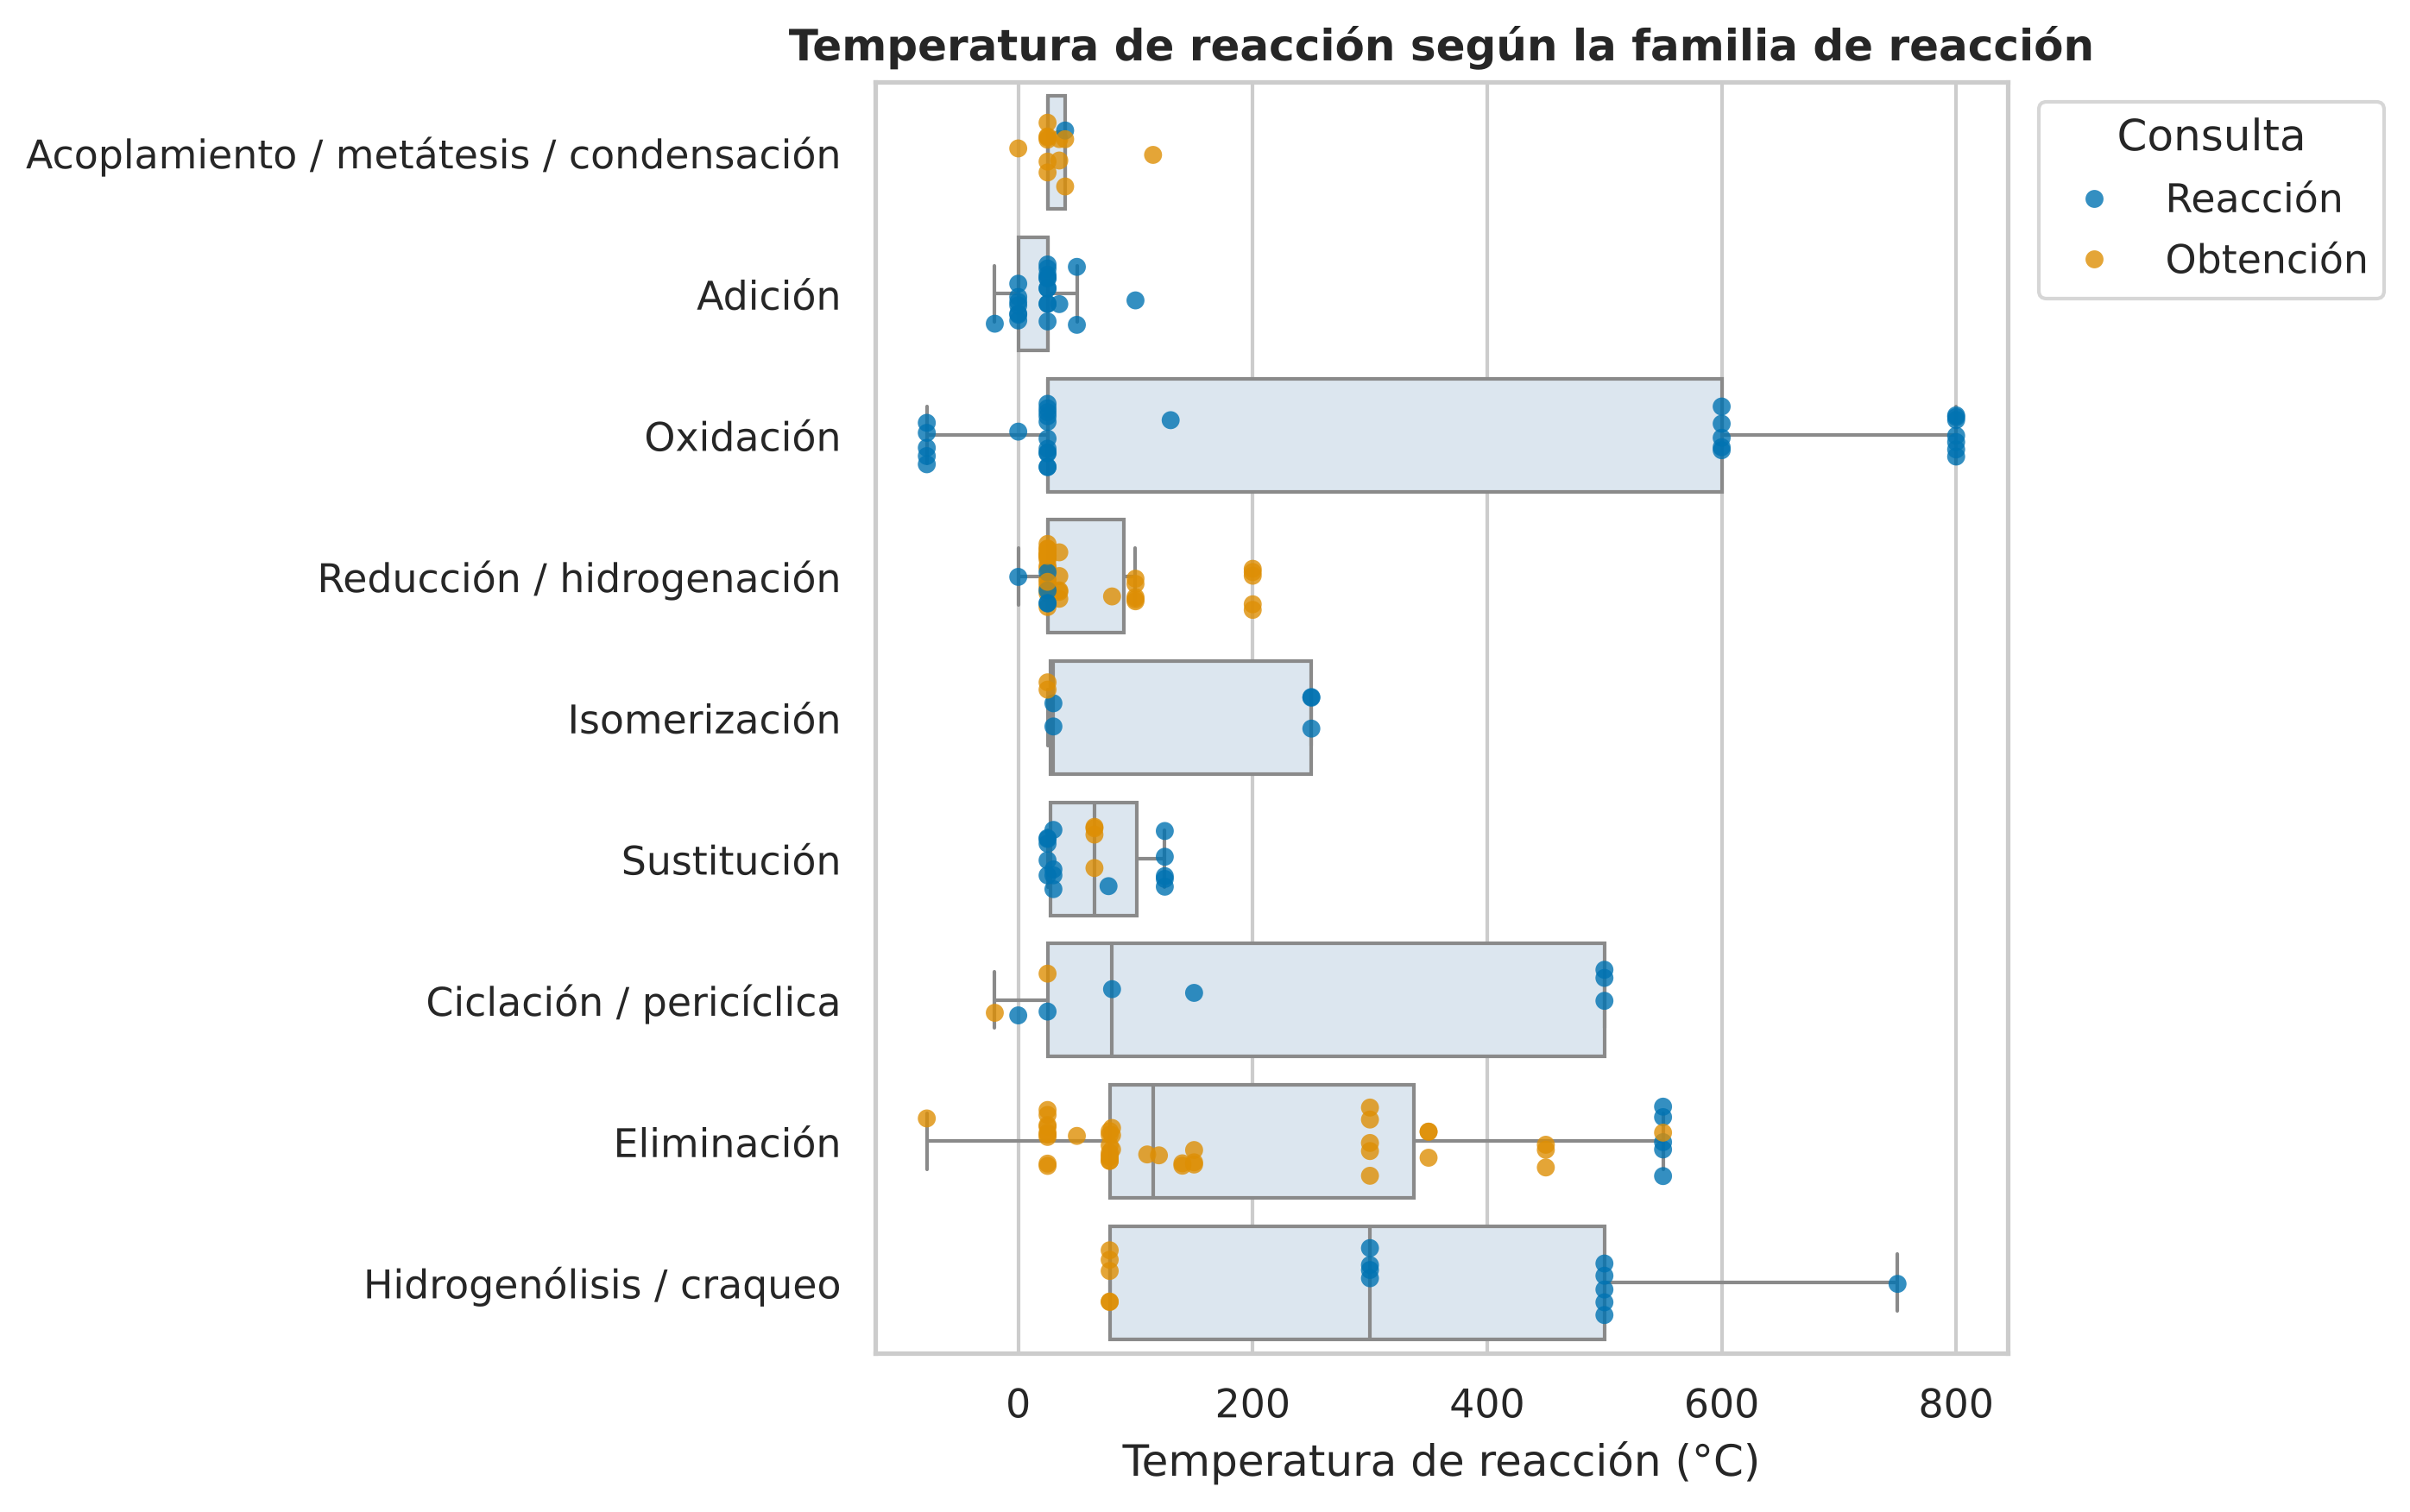
\includegraphics[width=\columnwidth]{12_box_T_por_familia.png}
\caption{Temperatura de reacci\'on seg\'un la familia de reacci\'on.}
\label{fig:box-t}
\end{figure}

\subsection{Reacciones frente a obtenciones}
La figura~\ref{fig:barras} explica el valor $V=0{,}76$ entre familia y tipo de consulta: la adici\'on (22) y la oxidaci\'on (30) aparecen solo como reacciones, mientras que la eliminaci\'on (41 de 46), la reducci\'on e hidrogenaci\'on (34 de 39) y el acoplamiento (12 de 13) son sobre todo obtenciones, porque los alquenos se obtienen por eliminaci\'on y los alcanos por reducci\'on o hidrogenaci\'on. Por tanto, la asociaci\'on no es un hallazgo estad\'istico independiente sino la consecuencia de la qu\'imica del grupo funcional.

\begin{figure}[!htbp]
\centering
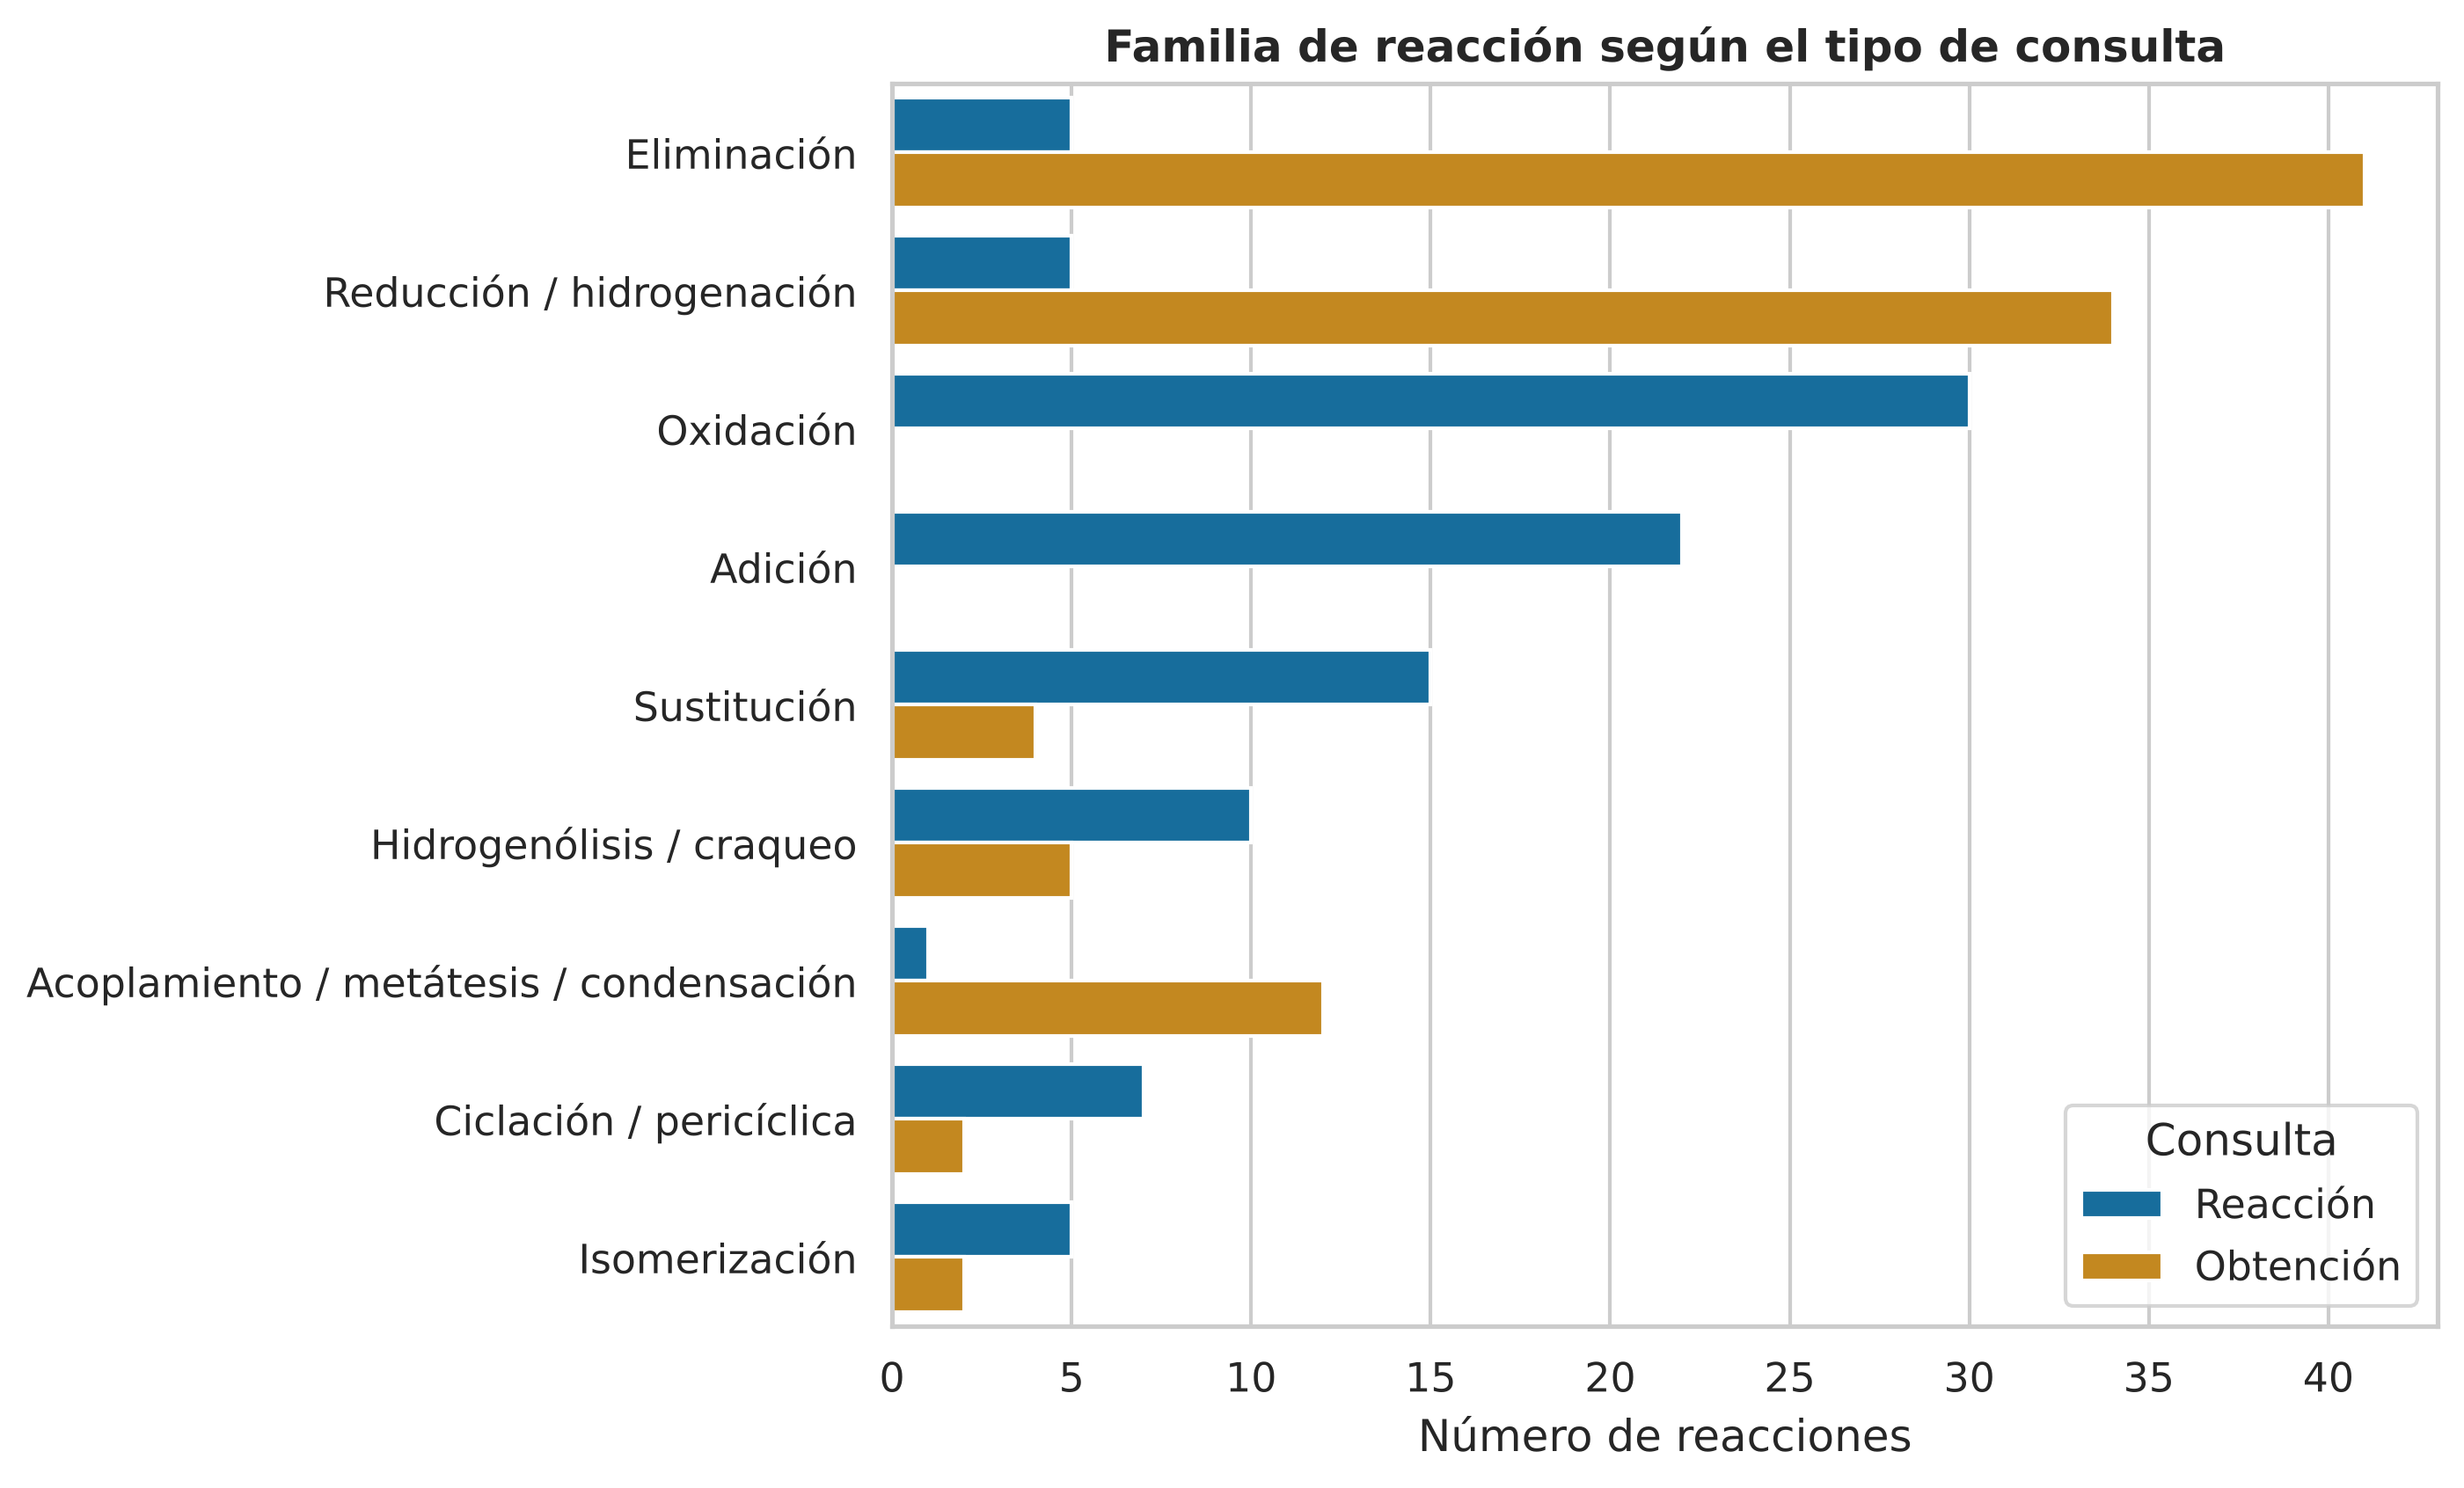
\includegraphics[width=\columnwidth]{14_barras_familia_consulta.png}
\caption{N\'umero de registros por familia de reacci\'on seg\'un el tipo de consulta.}
\label{fig:barras}
\end{figure}

En la figura~\ref{fig:ecdf} se compara la temperatura. La mediana de las reacciones es 30\,\textdegree C y la de las obtenciones 65\,\textdegree C, pero la cola de las reacciones llega mucho m\'as lejos: su percentil 90 es 600\,\textdegree C frente a 300\,\textdegree C, y 26 de los 30 registros a 400\,\textdegree C o m\'as son reacciones (combusti\'on, craqueo y reformado). Las curvas se cruzan: las reacciones comienzan m\'as ``fr\'ias'' pero terminan mucho m\'as ``calientes''. Por eso la prueba de Mann-Whitney no encuentra diferencia en el nivel central ($p=0{,}88$), pero la prueba de Levene s\'i la encuentra en la dispersi\'on (desviaci\'on est\'andar de 268 frente a 116\,\textdegree C, $p=2{,}5\times10^{-5}$). H4 se confirma entonces solo en parte.

\begin{figure*}[!t]
\centering
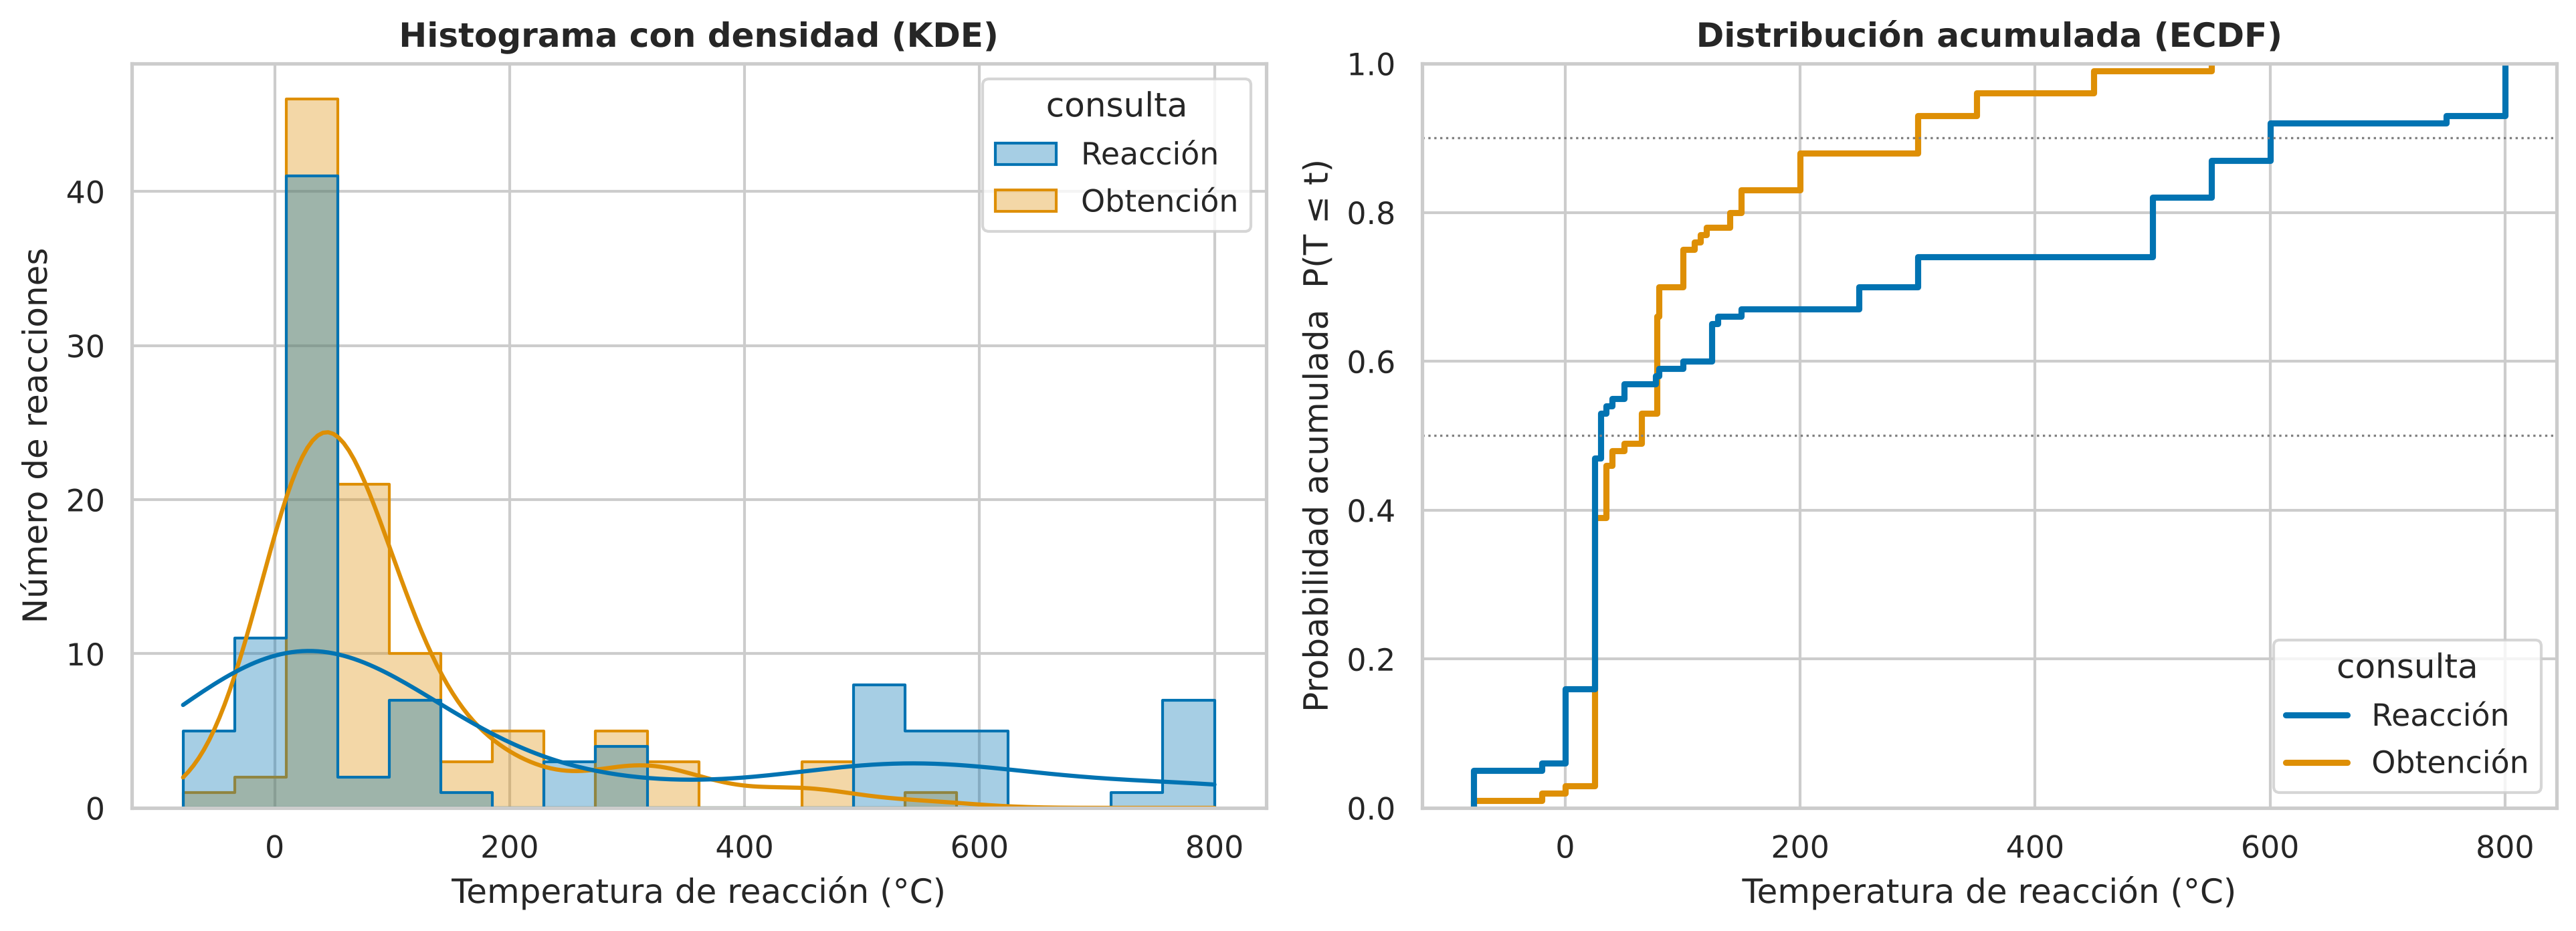
\includegraphics[width=0.92\textwidth]{13_hist_ecdf_temperatura.png}
\caption{Histograma con densidad (izquierda) y distribuci\'on acumulada (derecha) de la temperatura de reacci\'on, seg\'un el tipo de consulta.}
\label{fig:ecdf}
\end{figure*}

\subsection{Valores at\'ipicos}
Los valores at\'ipicos de la base no son errores sino sustancias o reacciones realmente distintas, por lo que se conservaron. De los 30 at\'ipicos de temperatura de reacci\'on (m\'as de 369\,\textdegree C), 27 corresponden a 500\,\textdegree C o m\'as y son combusti\'on, craqueo, deshidrogenaci\'on, reformado y pir\'olisis. En el punto de fusi\'on destacan cinco sales de sodio de \'acidos carbox\'ilicos (290--320\,\textdegree C), compuestos i\'onicos que no se parecen a las mol\'eculas covalentes del resto de la tabla; en la presi\'on de vapor, el \ce{CO2} (56\,500\,mmHg) de las combustiones completas; y en la densidad, los derivados dibromados (1,95--1,98\,g/cm$^3$). Tres registros de acetatos a 450\,\textdegree C (R120, R160 y R199) conviene verificarlos en SciFinder. Como estos valores pesan mucho en una correlaci\'on de Pearson, se utiliz\'o Spearman en lugar de eliminar datos.

\subsection{Contraste de las hip\'otesis}
La tabla~\ref{tab:hipotesis} resume las pruebas. H1, H2 y H3 se confirman y H4 solo en parte. En las pruebas de chi-cuadrado entre 22\,\% y 83\,\% de las celdas tienen frecuencia esperada menor que 5, as\'i que los valores $p$ son aproximados y la cifra m\'as robusta es el tama\~no de la asociaci\'on ($V$).

\begin{table*}[!t]
	\centering
	\footnotesize
	\begin{tabular}{|c|l|l|c|l|c|c|}
		\hline
		\textbf{Hip.} & \textbf{Prueba} & \textbf{Variables} & \textbf{Estad\'istico} & \textbf{Tama\~no de efecto} & \textbf{$p$} & \textbf{Decisi\'on} \\
		\hline
		H1 & Spearman & PM -- $T_{eb}$ & $\rho=0{,}82$ & $\rho^2=0{,}67$ & $2\times10^{-45}$ & Se confirma \\
		H1 & Spearman & PM -- $P_{vap}$ & $\rho=-0{,}80$ & $\rho^2=0{,}65$ & $5\times10^{-44}$ & Se confirma \\
		H1 & Spearman & $T_{eb}$ -- $P_{vap}$ & $\rho=-0{,}99$ & $\rho^2=0{,}98$ & $5\times10^{-153}$ & Se confirma \\
		H2 & $\chi^2$ & Familia -- medio & $\chi^2=193{,}0$ & $V=0{,}53$ & $2\times10^{-28}$ & Se confirma \\
		H2 & $\chi^2$ & Familia -- catalizador & $\chi^2=310{,}0$ & $V=0{,}47$ & $5\times10^{-40}$ & Se confirma \\
		H2 & $\chi^2$ & Familia -- solvente & $\chi^2=144{,}7$ & $V=0{,}45$ & $3\times10^{-19}$ & Se confirma \\
		H3 & Kruskal-Wallis & $T_{rxn}$ por familia & $H=49{,}3$ & $\varepsilon^2=0{,}22$ & $6\times10^{-8}$ & Se confirma \\
		H3 & Kruskal-Wallis & $T_{rxn}$ por catalizador & $H=21{,}9$ & $\varepsilon^2=0{,}08$ & $1{,}3\times10^{-3}$ & Se confirma \\
		H3 & Kruskal-Wallis & $T_{rxn}$ por solvente & $H=98{,}8$ & $\varepsilon^2=0{,}49$ & $3\times10^{-21}$ & Se confirma \\
		H4 & Mann-Whitney & $T_{rxn}$: reacci\'on frente a obtenci\'on & $U=5059$ & medianas 30 y 65\,\textdegree C & 0,88 & No hay diferencia \\
		H4 & Levene & Dispersi\'on de $T_{rxn}$ & $W=18{,}6$ & desv. est. 268 y 116\,\textdegree C & $2{,}5\times10^{-5}$ & Hay diferencia \\
		H4 & $\chi^2$ & Familia -- consulta & $\chi^2=123{,}1$ & $V=0{,}76$ & $7\times10^{-23}$ & Hay diferencia \\
		\hline
	\end{tabular}
	\captionsetup{width=\textwidth, justification=justified}
	\caption{Resultados de las pruebas de hip\'otesis ($n=200$, salvo $n=184$ para PM--$T_{eb}$ y $T_{eb}$--$P_{vap}$ y $n=189$ para PM--$P_{vap}$).}
	\label{tab:hipotesis}
\end{table*}

\section{Conclusiones y Perspectiva}
Del an\'alisis de los 200 registros se concluye lo siguiente.
\begin{enumerate}
\item El punto de ebullici\'on aumenta con el peso molecular ($\rho=0{,}82$) y la presi\'on de vapor disminuye ($\rho=-0{,}80$); entre ellas hay una relaci\'on casi perfecta ($\rho=-0{,}99$), por lo que son pr\'acticamente redundantes. En los alcanos lineales cada $-\mathrm{CH_2}-$ suma entre 27 y 33\,\textdegree C al punto de ebullici\'on y la ramificaci\'on lo reduce.
\item La familia de reacci\'on organiza las condiciones: se asocia con el medio ($V=0{,}53$), el catalizador ($V=0{,}47$) y el solvente ($V=0{,}45$) con patrones coherentes con los mecanismos (eliminaci\'on en medio b\'asico, sustituci\'on radicalaria en medio apolar, hidrogenaci\'on con metal soportado, isomerizaci\'on en medio \'acido).
\item La temperatura de reacci\'on tiene dos reg\'imenes: 51,5\,\% de los registros ocurre a 40\,\textdegree C o menos y un grupo de reacciones t\'ermicas se hace entre 400 y 800\,\textdegree C. No depende de las propiedades f\'isicas de la sustancia asociada.
\item Reacciones y obtenciones no difieren en la temperatura mediana, pero s\'i en el tipo de transformaci\'on ($V=0{,}76$) y en la dispersi\'on de la temperatura.
\item La sustancia consultada y su clase no determinan las condiciones ni el peso molecular de las sustancias asociadas ($\eta=0{,}08$): lo que decide es el mecanismo y el grupo funcional.
\end{enumerate}

Entre las limitaciones est\'an el tama\~no de la muestra ($n=200$), las celdas con frecuencia esperada baja en varias tablas de contingencia, el pKa casi vac\'io, el techo artificial de 760\,mmHg para los gases y el hecho de que una correlaci\'on no implica causalidad. Como perspectiva, se propone contrastar los 200 registros con m\'as fuentes, ampliar el conjunto a otras familias de hidrocarburos, probar modelos multivariados (por ejemplo, regresi\'on log\'istica para predecir el medio a partir de la familia y el catalizador) y llevar las relaciones encontradas a la presentaci\'on interactiva en Power BI.

\section{Declaración}
\fontsize{11}{13}\selectfont

\textbf{Conflicto de intereses: } los autores declaran que no tienen conflictos de intereses.

\textbf{Contribuci\'on de los autores:}
Jorge Nicol\'as M\'endez Castellanos: an\'alisis gr\'afico y estad\'istico en Python, visualizaci\'on y redacci\'on del informe. Laura Alejandra Parra y Gabriela Santamar\'ia: [completar seg\'un el reparto del grupo].

% Example for references section

\printbibliography  % Use BibLaTeX for printing bibliography

\end{document}
